% !TEX program = xelatex
\documentclass[11pt, a4paper]{article}

\usepackage{fontspec}
\setmainfont{Times New Roman}[Ligatures=TeX]
\usepackage[space]{xeCJK}
\IfFontExistsTF{Batang}{%
  \setCJKmainfont{Batang}
  \setCJKsansfont{Malgun Gothic}
  \setCJKmonofont{Malgun Gothic}
}{%
  \setCJKmainfont{AppleMyungjo}[AutoFakeBold=2]
  \setCJKsansfont{Apple SD Gothic Neo}
  \setCJKmonofont{Apple SD Gothic Neo}
}

\usepackage[margin=2.5cm]{geometry}
\usepackage{setspace}
\onehalfspacing

\usepackage{booktabs}
\usepackage{array}
\usepackage{longtable}
\usepackage{amsmath, amssymb}
\usepackage{graphicx}
\usepackage{float}
\usepackage[font=small, labelfont=bf, textfont=it]{caption}
\renewcommand{\arraystretch}{1.25}

\usepackage{listings}
\lstset{
  basicstyle=\ttfamily\small,
  breaklines=true,
  frame=single,
  xleftmargin=1em,
  framexleftmargin=0.5em,
  numbers=none,
  aboveskip=1em,
  belowskip=1em,
  columns=fullflexible,
}

\usepackage{xcolor}
\usepackage{tikz}
% 근거 기록을 찾지 못해 비워 둔 자리
\newcommand{\blank}[1]{\fcolorbox{red!60!black}{yellow!20}{\small 미기입: #1}}
\usepackage[colorlinks=true, linkcolor=blue!60!black, citecolor=blue!60!black, urlcolor=blue!60!black]{hyperref}

\title{%
  상호작용 서사에서의 감정 궤적 이탈 측정\\
  \large --- \textit{The Etched Mutation} 시스템과 메트릭 ---\\[0.8em]
  \normalsize Measuring Emotional Trajectory Divergence in Interactive Narrative:\\
  The Etched Mutation System and Its Metrics
}
\author{박도한 (Dohhan Park)\\ \small The Etched Mutation}
\date{Working Draft v0.5 --- 2026-11-20}

\begin{document}
\maketitle

\begin{abstract}
\noindent 상호작용 서사에서 서로 다른 체험자는 서로 다른 경험을 하지만, 그 ``다름''은 대부분 플롯 분기의 차이로만 기술되어 왔다. 본 논문은 \textbf{감정 궤적(emotional trajectory)을 상호작용 서사의 일차 차원으로 두는} 시스템 \textit{The Etched Mutation (TEM)}과, 체험자 궤적이 작가 원본 궤적으로부터 이탈하는 양상을 두 가지 분리 가능한 양식 --- \textbf{drift (방향 이탈)}과 \textbf{fixation (단일점 수렴)} --- 으로 측정하는 오염 벡터(contamination vector), 그리고 궤적 형태의 유사도를 실시간으로 산출하는 별이엔진 V4(Byeori Engine V4)의 정렬도(alignment) 메트릭을 제시한다. 본 시스템은 명시적 분기 구조 없이 매 턴 체험자의 감정 상태에 따라 접근 가능한 장면 집합(accessible pin set)을 계산하며, 공명(resonance)에 도달한 체험자의 궤적은 다음 체험자를 위한 해석 조각(\textit{trajectory bridge})으로 자동 변환된다. 단일 작품에 대한 페르소나 시뮬레이션(페르소나 15명, 39회차, 193 장면-플레이)으로 정렬도의 장면별 유사도 성분(level)을 시범 평가하며, 성격 특질(개방성·친화성·외향성)이 정렬도와 양의 상관을 보임($r = 0.55$--$0.63$, $n=15$; 다섯 특질에 대한 다중비교 보정 뒤에는 유의 문턱에 못 미침)과 동시에 LLM 시뮬레이션 독자가 과공명(over-resonance) 천장 편향을 보인다는 계측기의 한계를 함께 보고한다. 나아가 공개 알파에서 수집된 3인 파일럿 인간 관찰(21 장면-플레이)이 이 경계와 정합함을 예비적으로 확인한다 --- 시뮬레이션에 부재하던 낮은 꼬리($<0.25$)가 인간 분포에서 실재했다(14.3\%). 궤적 형태 성분(shape)과 오염 벡터는 구현되어 있으나 본 논문에서 수치로 평가되지 않았으며, 그 간극을 \S5.7에 표로 적는다. 본 논문이 내놓는 것은 거대 이론의 증명이 아니라, 실제로 작동하는 \textbf{측정 장치와 체험 시스템}이다.

\medskip
\noindent\textbf{키워드:} 상호작용 서사, 감정 궤적, 정렬도, 오염 벡터, 궤적 비교, 정서 컴퓨팅, 독자 궤적
\end{abstract}

\medskip
\noindent{\small\textbf{판 이력.} v0.5는 v0.4(2026-08-04)에 ICIDS 2026 Late-Breaking Works 심사(2026-10-07, 불채택)의 지적을 반영한 판이다. 새로 넣거나 고친 곳: 작품과 체험 서술(\S3.1), 접근 중심 이동 그림(그림~\ref{fig:center}), 선행 연구 보강(\S2.4), 표본 단위 표기 정정(\S5.1), 상관의 신뢰구간과 다중비교 보정(\S5.3), 제목이 약속한 것과 실제로 잰 것(\S5.7), 참가자와 동의(\S7), 재현 세부(부록~\ref{app:repro}). 노란 상자 ``미기입''은 근거 기록을 찾지 못해 비워 둔 자리이며 지어내어 채우지 않았다.\par}

% ════════════════════════════════════════
\section{서론}

\subsection{문제 설정 --- 체험자의 ``다름''을 어떻게 측정할 것인가}

상호작용 서사(interactive narrative)의 핵심 약속은 체험자마다 다른 경험을 제공한다는 것이다. Janet Murray(1997)의 \textit{Hamlet on the Holodeck} 이래, 이 약속을 구현하는 도구는 Twine, Ink, Articy:Draft, 나아가 StoryAssembler와 Versu 등 다양하게 발전해 왔다. 그러나 대부분의 도구는 \textbf{플롯 분기(branching plot)를 통한 경로의 다양성}에 집중해 왔으며, 체험자가 서사를 관통하며 겪는 \textbf{감정의 궤적}은 명시적으로 추적되지 않았다.

이 공백은 정서 컴퓨팅(affective computing) 쪽에서도 정확히 메워지지 않는다. 감정의 정량적 모델은 VAD(Russell \& Mehrabian, 1977), PANAS(Watson et al., 1988), 감정 단어 규범(Warriner et al., 2013)으로 확립되어 있고, 감정의 시간적 패턴이 경험의 질을 예측한다는 TIES(Temporal Interpersonal Emotion Systems; Butler, 2011, 2017) 프레임워크와 그 계산적 구현인 CompTIES(Butler et al., 2017)가 있지만, 이들은 기본적으로 \textbf{관찰된 감정 데이터를 사후에 분석}하는 도구이며, 상호작용 서사 내부의 \textbf{실시간 궤적 비교}에는 적용되지 않는다. Reagan et al.(2016)은 서사의 감정 arc가 6개의 대표 형태로 수렴함을 보였으나, 이는 \textbf{작품과 작품을 견주는} 비교였을 뿐, \textbf{같은 작품을 체험한 두 사람의 궤적}을 견주지는 않는다.

본 논문이 답하려는 질문은 다음과 같다:
\begin{itemize}
  \item \textbf{R1.} 플롯 분기 없이, 체험자의 감정 궤적만으로 작동하는 상호작용 서사 접근 모델이 가능한가?
  \item \textbf{R2.} 체험자 궤적이 작가 원본 궤적으로부터 이탈하는 양상을 \textbf{정량적으로}, 그리고 \textbf{서로 다른 양식으로 분리하여} 측정할 수 있는가?
  \item \textbf{R3.} 특정 정서적 지향점(공명)에 도달한 체험자의 궤적이 다음 체험자를 위한 \textbf{해석 조각}으로 자동 변환되는 메커니즘이 구현 가능한가?
\end{itemize}

\subsection{기여}

본 논문은 세 가지 기여를 제시하며, 각 기여는 기존 연구가 비워 둔 특정 지점을 겨냥한다.

\textbf{첫째, 시스템적 기여.} \textit{The Etched Mutation (TEM)} --- 감정 벡터를 씬(scene)의 일차 속성으로 두고, 매 턴 체험자 감정 상태에 따라 접근 가능 씬 집합을 계산하는 인터랙티브 서사 시스템. 기존 저작 도구(Twine, Ink, Articy)가 명시적 플롯 분기 조건식으로 경로를 가르는 데 반해, TEM은 분기 조건식 없이 체험자 감정 상태와 씬 원본 감정 사이의 거리만으로 다음 경로를 결정한다. 나아가 전이 패턴(transition pattern)은 접근 공간의 \textit{반경}이 아니라 \textit{중심}을 이동시킨다. 같은 정렬도라도 패턴이 다르면 다른 씬으로 이어진다(\S3.3).

\textbf{둘째, 방법론적 기여.} 두 가지 계산 가능한 메트릭. (1)~\textbf{별이엔진 V4 정렬도} --- 체험자 감정 시퀀스와 작가 원본 감정 시퀀스의 형태 유사도를 실시간으로 산출. 정서 컴퓨팅의 대인 감정 비교(TIES/CompTIES)가 관찰 데이터를 \textit{사후 분석}하는 데 반해, 별이엔진은 감정의 전체 강도(level)를 제거하고 변화의 \textit{형태(shape)}만 비교하는 정렬도를 인터랙티브 서사 내부에서 매 턴 실시간으로 산출한다. (2)~\textbf{오염 벡터} --- 궤적 이탈을 \textbf{drift (방향성 누적 이탈)}과 \textbf{fixation (단일 귀인·감정으로의 과도한 수렴)} 두 축으로 분리 측정. 두 축은 동일 총 이탈량이라도 체험적으로 다른 양상을 구분한다.

\textbf{셋째, 시범 평가.} 단일 작품 193 장면-플레이(39회차) 규모의 페르소나 시뮬레이션으로 정렬도의 장면별 유사도 성분(level)이 페르소나 성격에 따라 갈리는지를 보고, 동시에 시뮬레이션 계측기 자체의 측정된 한계(과공명 천장 편향)를 보고한다. 평가 범위가 level 성분에 한정된다는 점은 \S5.7에 따로 적는다.

% ════════════════════════════════════════
\section{관련 연구}

\subsection{기억의 구성적 성격과 변형의 메커니즘}

기억 변형 현상에 대한 인지심리학의 축적은 두껍다. Bartlett(1932)의 고전적 연구는 기억이 저장소에서 인출되는 것이 아니라 \textbf{매번 재구성}된다는 것을 밝혔다. Nader et al.(2000)의 재고화(reconsolidation) 연구는 회상이 기억을 불안정화시키고 현재 맥락과 함께 재저장하는 분자적 메커니즘을 밝혔으며, Bridge \& Paller(2012)는 인간에서도 동일 현상을 확인했다. Loftus \& Palmer(1974)와 Loftus(2005)의 오정보 효과(misinformation effect)는 사후 정보가 기억을 체계적으로 왜곡함을, Roediger \& McDermott(1995)의 DRM 패러다임은 실제로 경험하지 않은 사건의 거짓 기억 생성을, Johnson et al.(1993)의 출처 모니터링 연구는 기억 출처의 체계적 혼동을 보였다. Bower(1981), Levine(1997), Tversky \& Marsh(2000), Schooler \& Engstler-Schooler(1990), Pasupathi(2001), Hirst \& Echterhoff(2012), Patihis \& Loftus(2016) 등은 감정 상태·사회적 청자·언어화·치료적 상상이 회상 내용을 \textbf{비무작위적으로} 왜곡함을 밝혔다.

그러나 이 연구들은 대체로 서로 떨어진 \textbf{개별 현상으로 다뤄져 왔다}. 본 논문은 이들을 하나로 묶는 통합 이론을 제안하지 않는다. 본 논문이 다루는 것은 이 변형들 중 \textbf{감정 궤적의 이탈}이라는 한 단면을, 인터랙티브 서사 안에서 실시간으로 측정 가능한 양으로 만드는 장치이다.

\subsection{감정 측정과 대인 비교}

감정의 정량 모델은 VAD(Russell \& Mehrabian, 1977), Ekman(1992)의 기본 정서, PANAS(Watson et al., 1988), 감정 단어 규범(Warriner et al., 2013)으로 확립되어 있다. 두 사람의 감정 경험을 비교하는 연구로는 감정 수렴(Anderson et al., 2003)이 있고, Butler(2011, 2017)의 TIES 프레임워크는 감정의 \textbf{동적 패턴}이 관계 질을 예측함을 이론화했으며, Butler et al.(2017)의 CompTIES는 이를 \textbf{coupled oscillator 모델}로 계산적으로 구현했다.

그러나 CompTIES는 비디오 rating dial 기록에 모델을 \textbf{사후에 피팅}하는 관찰 데이터 분석 도구이며, 실시간 인터랙티브 환경에서 체험자의 감정 입력에 즉각 반응하며 원본 궤적과 비교하는 도구는 확립되어 있지 않다. 본 논문의 별이엔진 V4(\S4.1)는 TIES의 핵심 원리 --- \textit{궤적의 동적 패턴이 수준(level)과 독립적으로 유사성을 예측한다} --- 를 상호작용 서사의 \textbf{실시간 내부 엔진}으로 이식한 첫 시도이다.

\subsection{상호작용 서사와 감정 축의 부재}

Janet Murray(1997), Marie-Laure Ryan(2001), Espen Aarseth(1997)의 이론적 작업은 상호작용 서사의 철학적 기반을 놓았다. 저작 도구 측면에서 Twine은 명시적 분기 기반, Ink(Inkle)는 변수·상태 기반 분기, Articy:Draft는 작가 노드 저작에 중점을 둔다. 학술 시스템으로 StoryAssembler(Garbe et al., 2019)와 Versu(Evans \& Short, 2014)가 있다. 공통적으로, \textbf{감정이 서사 상태의 일차 차원(first-class dimension)으로 다뤄지지 않는다.} 본 논문은 감정 벡터를 씬의 일차 속성으로 두고, 체험자의 현재 감정 상태를 \textbf{접근 가능 씬 집합의 직접 결정 인자}로 사용한다(\S3.3).

\subsection{분기 없는 서사 접근: 드라마 매니지먼트 계보}

``작가가 명시적 분기 그래프를 그리지 않아도 시스템이 다음 서사 단위를 선택한다''는 발상 자체는 새롭지 않다. Façade(Mateas \& Stern, 2003, 2005)는 서사를 조각(beat) 단위로 구성하고, 드라마 매니저(drama manager)가 작가가 명시한 미학적 목표 --- Aristotelian 긴장 곡선 --- 를 향해 다음 beat를 실시간으로 선택한다. 이 계보는 탐색 기반 드라마 매니지먼트(Weyhrauch, 1997)로 형식화되었고, PaSSAGE(Thue et al., 2007)는 여기에 \textbf{플레이어 모델링}을 더해 체험자를 유형으로 분류한다. 이들은 오늘날 경험 관리(experience management; Riedl \& Bulitko, 2013)라는 우산 아래 묶인다. TEM은 이 계보와 \textbf{분기 그래프 없이 다음 단위를 선택한다}는 성질을 공유한다.

그러나 세 지점에서 갈라지며, 이 차이가 본 논문의 기여를 규정한다. 첫째, \textbf{목적 함수의 방향이 반대다.} 드라마 매니저는 목표 궤적을 향해 최적화하며 체험자의 이탈을 되돌려야 할 오차로 취급한다. TEM은 어떤 목표 궤적으로도 조향하지 않는다. 작가의 감정 궤적은 \textbf{최적화 대상이 아니라 측정 기준선}이며, 거기서의 발산 그 자체가 렌더링되는 내용물이다(\S4.2). 둘째, \textbf{잠재 플레이어 모델이 없다.} 별이엔진은 체험자 감정 시퀀스와 작가 시퀀스의 기하적 관계를 매 턴 계산할 뿐 분류도 추천도 하지 않는다(``엔진은 판단하지 않는다. 관찰하고 보고할 뿐''; \S4). 셋째, \textbf{선택이 이루어지는 공간이 다르다.} TEM의 접근 가능 씬 집합은 감정 다양체(affective manifold) 위의 이웃이며, 그 이웃의 \textbf{중심이 전이 패턴에 따라 이동}한다(\S3.3).

가장 검증 가능한 차이는 \textbf{데이터 구조 수준의 분기 소멸}이다. beat 기반 드라마 매니저조차 beat에 선·후행 조건을 부여하므로 내부에는 부분적 플롯 그래프가 남는다. TEM의 \texttt{choice}에는 \texttt{next\_scene\_id} 열이 \textbf{존재하지 않으며}(\S3.2), 가지치기할 플롯 그래프 자체가 없다. 분기를 숨긴 것이 아니라 스키마 차원에서 아예 없앤 것이다. 이는 비유가 아니라 데이터 모델에서 그대로 확인된다.

감정이나 관객 반응을 서사 생성의 동력으로 삼은 선행 시스템도 이 계보에 놓인다. FearNot!(Aylett et al., 2005)은 평가(appraisal) 기반 감정 구조를 가진 자율 캐릭터들의 상호작용에서 각본 없는 서사가 창발하도록 한 따돌림 예방 교육 시스템이다. 거기서 감정은 \textit{캐릭터}의 내부 상태이고 서사를 만들어 내는 원인이다. TEM에서 감정은 \textit{체험자}의 입력이며, 작가 궤적과의 관계가 측정되는 대상이다. Terminal Time(Mateas et al., 2000)은 관객의 박수 응답으로 다음 내용을 고르고 기울여 이념적으로 편향된 역사 다큐멘터리를 생성한다. 관객 반응이 미리 그려 둔 분기를 고르는 것이 아니라 생성 전체의 기울기를 정한다는 점에서 TEM과 가깝다. 차이는 Terminal Time이 관객 집단의 응답을 하나의 편향 모델로 모아 작품을 그쪽으로 기울이는 데 반해, TEM은 체험자 한 사람의 궤적을 요약하지 않고 그대로 보존하며 작가 궤적과의 차이를 기록한다는 것이다.

\subsection{체험자 흔적의 다음 체험자로의 전달}

체험자의 흔적이 다음 체험자에게 전해지는 메커니즘의 기존 형태는 세 부류다. 첫째, FromSoftware의 \textit{Soulsborne} 시리즈 메시지 시스템은 공간 위치에 플레이어 메시지를 익명으로 남긴다(FromSoftware, 2011). 둘째, Hypothesis(hypothes.is)는 웹 페이지에 다수 독자의 주석을 중첩한다. 셋째, Genius.com은 가사에 해석을 중첩하되 \textbf{인기도 기반}으로 정렬한다. TEM의 궤적 브릿지(\S3.5)는 첫 번째에 가장 가까우나 결정적 차이가 있다. Soulsborne 메시지는 \textbf{공간 좌표}에 붙지만, 궤적 브릿지는 \textbf{감정 축}에 붙는다. 또한 Genius의 인기도 정렬을 명시적으로 거부한다 --- 노출 조건은 체험자 감정 상태와의 \textbf{정렬도}이지 누적 좋아요가 아니다.

\subsection{본 논문의 위치}

\begin{table}[H]
\centering
\caption{선행 연구와 TEM의 관계}
\small
\begin{tabular}{p{4.6cm} p{4.0cm} p{5.2cm}}
\toprule
\textbf{선행 연구} & \textbf{기여} & \textbf{TEM과의 관계} \\
\midrule
Bartlett(1932), Nader et al.(2000) 등 & 기억 변형 메커니즘 규명 & 배경으로만 참조 --- 인지 메커니즘 주장 안 함 \\
Butler(2011, 2017) TIES / CompTIES(2017) & 감정 동적 패턴 사후 분석 & 별이엔진이 실시간 인터랙티브로 확장 \\
Reagan et al.(2016) & 서사 감정 arc 형태 6종 & 작품 간 $\rightarrow$ 체험자 간 비교로 확장 \\
Twine, Ink, Articy & 플롯 분기 저작 & 분기 없이 감정 궤적으로 접근 결정 \\
Façade(2005), PaSSAGE(2007) & 분기 그래프 없는 서사 선택 & 발산을 최적화 대상 $\rightarrow$ 렌더링 내용물로 전환 \\
FearNot!(2005), Terminal Time(2000) & 캐릭터 감정·관객 반응이 서사를 생성 & 캐릭터 감정·집단 편향 $\rightarrow$ 체험자 개인 궤적의 측정 \\
Soulsborne, Hypothesis & 독자 흔적 중첩 & 공간$\rightarrow$감정 축, 인기도$\rightarrow$정렬도 기반 \\
\bottomrule
\end{tabular}
\end{table}

% ════════════════════════════════════════
\section{The Etched Mutation (TEM)}

\subsection{개요}

TEM은 두 가지 모드로 작동하는 상호작용 서사 시스템이다. \textbf{Record 모드}에서 작가는 자신의 기억을 AI와의 대화를 통해 씬 단위로 구조화한다. \textbf{Play 모드}에서 체험자는 타인의 기억을 씬 단위로 체험하며, 매 턴 자신의 감정 입력을 제공한다. Strata 모드는 전체 기억을 3D 감정 지형으로 조망한다. 시스템은 vanilla JavaScript ES6 모듈, Three.js (3D), Supabase (인증·DB·Edge Functions), HRTF 기반 Web Audio API로 구현되어 있으며, vitest 기반 결정론적 회귀 테스트가 상시 실행된다.

\subsubsection*{관객의 한 회차 --- 관객은 무엇을 하는가}

작가는 기억 하나를 씬들로 저작한다. 관객의 한 회차는 다음과 같이 흐른다(인간 파일럿 자료가 모인 지형 무대 기준).
\begin{enumerate}
  \item 관객은 안개 속에서 지금 접근 가능한 씬 가운데 하나로 걸어간다. 전체 지도는 보이지 않는다.
  \item 씬에는 글과 소리, 그리고 \textbf{유령}(앞선 통과자들의 잔향)이 있다. 유령의 말은 흔들리는 자리에서 끊겨 있고, 관객은 그 뒤를 \textbf{이어 쓴다}.
  \item 관객이 쓴 말은 분류기를 거쳐 감정 축 위의 벡터로 기록된다.
  \item 그 벡터와 지금까지의 궤적으로부터 다음에 접근 가능한 씬 집합이 계산된다(\S3.3).
  \item 첫 씬(가장 앞 순서)은 프롤로그다. 유령이 없어 감정 입력이 없고 기록도 남지 않는다.
  \item 접근 가능한 씬이 0개가 되면 조용히 하나를 여는 대신 서사로 감싼 대체 경로가 열린다. 회차의 길이가 관객마다 다른 것은 실패나 벌이 아니라 이 구조의 결과다.
\end{enumerate}

\subsubsection*{평가에 쓰인 두 작품}

\textbf{MM23L 「당신에게」} --- 페르소나 시뮬레이션(\S5.1--5.4)이 읽은 작품. 죽은 이에게 쓰는 편지이며, 시뮬레이션 설계는 이 작품의 주제를 애도·애착·해리·환생으로 적고 있다. 시뮬레이션에 쓰인 씬은 순서 0--9의 열 개로, 씬 하나는 24--110자의 짧은 글이다(표~\ref{tab:scenes}). 작가가 씬마다 붙인 감정 분포는 2026-11-20 현재 DB 값이며, 이 값으로 193건의 정렬도를 다시 계산하면 저장된 값과 전부 일치한다(최대 차이 $<10^{-15}$).

\begin{table}[H]
\centering
\caption{MM23L 「당신에게」의 씬과 작가가 붙인 감정 (비중 상위 둘)}
\label{tab:scenes}
\small
\begin{tabular}{c c l p{5.6cm}}
\toprule
\textbf{순서} & \textbf{글자 수} & \textbf{작가가 붙인 주 감정} & \textbf{한 줄 요약} \\
\midrule
0 & 107 & 수치 0.35 · 고립 0.25 & \blank{작가 기입} \\
1 & 93 & 죄책감 0.40 · 두려움 0.20 & \blank{작가 기입} \\
2 & 110 & 혼란 0.30 · 두려움 0.25 & \blank{작가 기입} \\
3 & 24 & 무감각 0.35 · 죄책감 0.30 & \blank{작가 기입} \\
4 & 81 & 슬픔 0.35 · 그리움 0.25 & \blank{작가 기입} \\
5 & 80 & 죄책감 0.35 · 그리움 0.25 & \blank{작가 기입} \\
6 & 73 & 두려움 0.30 · 그리움 0.25 & \blank{작가 기입} \\
7 & 81 & 두려움 0.40 · 사랑 0.20 & \blank{작가 기입} \\
8 & 81 & 혼란 0.30 · 그리움 0.25 & \blank{작가 기입} \\
9 & 87 & 두려움 0.35 · 그리움 0.30 & \blank{작가 기입} \\
\bottomrule
\end{tabular}
\end{table}

시뮬레이션 독자는 위의 회차 흐름을 걷지 않는다는 점을 밝혀 둔다. 페르소나는 안개 속을 걷거나 유령의 말을 이어 쓰지 않고, 씬을 무작위 순서로 하나씩 건네받아 응답한다(부록~\ref{app:sim}).

\textbf{UNDW-001 「팬티만 입은 내여자」} --- 인간 파일럿(\S5.5)이 모인 작품. 13씬. 세 체험자의 21 장면-플레이가 모두 이 작품에서 나왔다. \blank{작품 소개 한 단락과 씬별 표 --- 작가 기입}

\subsection{데이터 모델}

TEM의 핵심 데이터 모델은 표~\ref{tab:datamodel}과 같다.

\begin{table}[H]
\centering
\caption{TEM 핵심 데이터 모델}
\label{tab:datamodel}
\small
\begin{tabular}{l p{6.4cm} p{4.4cm}}
\toprule
\textbf{엔티티} & \textbf{핵심 필드} & \textbf{의미} \\
\midrule
memory & id, code, title, meta.emotion\_entries & 작가가 기록한 기억 한 편 \\
scene & id, memory\_id, scene\_order, text, emotion\_vector, echo\_words, original\_emotion, text\_stage\_1/2/3 & 씬 한 개. emotion\_vector는 8축 \\
choice & id, scene\_id, emotion, intensity & \textbf{씬 내 선택지. 감정 결만 기록. next\_scene\_id 없음.} \\
play & id, memory\_id, curator\_id, trajectory\_data & 체험자 한 번의 플레이 궤적 \\
trajectory\_bridge & id, memory\_id, scene\_id, source\_run\_id, entry\_emotion, key\_passed\_scenes[], status & 공명 도달자 궤적의 자동 변환물 \\
author\_bridge & memory\_id, scene\_id, text & 작가가 쓴 정적 해석 조각 \\
\bottomrule
\end{tabular}
\end{table}

여기서 눈여겨볼 것은 \texttt{choices.next\_scene\_id}가 \textbf{존재하지 않는다}는 점이다. 빠뜨린 게 아니라 의도한 설계다. 선택지는 \textbf{체험자 감정 상태를 변화시키는 입력}일 뿐이며, 다음 씬은 감정 상태의 함수로 결정된다(\S3.3).

\subsection{감정 궤적 기반 Scene Navigation}

TEM의 접근 규칙은 다음과 같이 요약된다: \textit{매 턴, 체험자의 현재 감정 상태와 각 씬의 원본 감정 사이의 거리를 계산하고, 거리가 임계값 이내인 씬들을 접근 가능 씬 집합(\texttt{accessiblePinIds})으로 제시한다.} 구체적으로, 씬 $s$의 원본 감정 벡터 $o_s \in \mathbb{R}^8$과 체험자 현재 상태 $u_t \in \mathbb{R}^8$에 대해,
\begin{equation}
d(s, t) = 1 - \cos(u_t, o_s)
\end{equation}
의 값이 임계값 $\tau$ 이하인 씬을 후보로 삼고, 최근 방문 이력을 고려한 가중치로 정렬하여 상위 $k$개를 제시한다.

이 설계에서 중요한 것은 전이 패턴(transition pattern)이 접근 공간의 \textbf{반경이 아니라 중심}을 옮긴다는 점이다. echo\_follow는 중심을 원본 쪽으로, contradiction은 체험자 현재 감정의 반대쪽으로, avoidance는 중립 영역으로 옮긴다. 패턴이 반경만 조절한다면 엔진은 단순 룩업 테이블로 격하되고 만다. 그래서 패턴마다 중심 자체가 이동해야 한다. 이 설계의 결과로, \textbf{동일 작품을 체험한 두 사람이 완전히 다른 씬 시퀀스를 경험할 수 있다.} 이것이 본 논문이 측정하려는 ``다름''의 구체적 형태이다. 그림~\ref{fig:center}는 이 이동을 개념도로 보인다. 구현에 쓰인 비율과 반경은 부록~\ref{app:engine}에 있다.

\begin{figure}[H]
\centering
\begin{tikzpicture}[scale=1.0, every node/.style={font=\small}]
  \draw[gray!50, ->] (-6.6,-2.7) -- (6.5,-2.7);
  \draw[gray!50, ->] (-6.6,-2.7) -- (-6.6,5.3);
  \node[gray, anchor=north east] at (6.5,-2.75) {감정 공간 (개념도)};
  % scene pins
  \foreach \x/\y in {-5.6/2.6, -4.4/-1.6, -2.6/2.4, 3.0/2.6, 4.8/3.9, 5.4/0.6, 4.4/1.4, -5.9/-1.2, -0.6/2.9, 0.9/-2.2, -2.0/-1.7, 5.0/-2.2, -4.6/4.2}
    \fill[gray!55] (\x,\y) circle (1.6pt);
  % original and user
  \coordinate (O) at (-3.2,0.4);
  \coordinate (U) at (3.4,-1.4);
  \draw[dashed, gray] (O) -- (U);
  \fill[black] (O) circle (3pt);
  \node[anchor=east] at (-3.8,0.4) {씬 원본 감정 $o$};
  \fill[black] (U) circle (3pt);
  \node[anchor=west] at (3.6,-1.4) {체험자 감정 $u$};
  % centres on the o--u line
  \coordinate (E) at (-1.22,-0.14);
  \coordinate (B) at (0.1,-0.5);
  \coordinate (D) at (1.42,-0.86);
  \draw[blue!60!black, thick] (E) circle (0.45); \fill[blue!60!black] (E) circle (1.6pt);
  \node[blue!60!black, anchor=south east] at (-0.9,0.85) {echo\_follow (0.7 : 0.3)};
  \draw[blue!60!black, thin] (-1.22,0.85) -- (-1.22,0.31);
  \draw[green!45!black, thick] (B) circle (0.45); \fill[green!45!black] (B) circle (1.6pt);
  \node[green!45!black, anchor=south] at (0.3,0.1) {bridge (0.5 : 0.5)};
  \draw[orange!80!black, thick] (D) circle (0.45); \fill[orange!80!black] (D) circle (1.6pt);
  \node[orange!80!black, anchor=north] at (1.42,-1.45) {displacement (0.3 : 0.7)};
  % contradiction: reflection of u through the centroid of the pins
  \coordinate (G) at (1.0,1.6);
  \coordinate (C) at (-1.4,4.6);
  \fill[gray!70!black] (G) circle (2pt);
  \node[gray!70!black, anchor=west] at (1.2,1.65) {씬 무리의 중심};
  \draw[red!70!black, ->, dotted, thick] (U) -- (G) -- (C);
  \draw[red!70!black, thick] (C) circle (0.45); \fill[red!70!black] (C) circle (1.6pt);
  \node[red!70!black, anchor=west] at (-0.85,4.65) {contradiction (반대편)};
  % fixation
  \draw[black, thick, densely dashed] (O) circle (0.42);
  \node[anchor=north east] at (-2.6,-0.25) {fixation (지금 씬 근처)};
\end{tikzpicture}
\caption{전이 패턴에 따른 접근 중심의 이동(개념도, 실제 자료의 그림이 아님). 회색 점은 씬. 색 원은 패턴별 접근 공간이며, 원의 크기가 아니라 \textbf{자리}가 패턴마다 다르다. echo\_follow·bridge·displacement는 원본과 체험자를 잇는 선 위에서 섞는 비율이 다르고, contradiction은 체험자 감정을 씬 무리의 중심에 대해 뒤집은 자리에, fixation은 지금 씬 근처에 중심을 둔다. avoidance(감정 공백 영역)는 그림에서 생략했다.}
\label{fig:center}
\end{figure}

\subsection{Strata --- 3D 감정 지형}

strata는 모든 씬을 3차원 감정 공간에 배치하는 뷰이다. VAD 투영으로 $(x, z)$ 평면 위치를, 감정 강도로 $y$축 높이를 결정하며, AF(Attribution $\times$ Core Fear) 좌표계를 보조로 사용한다. 각 씬 핀에는 HRTF 기반 공간음향이 결합되어, 체험자가 1인칭으로 걸으면서 감정 지형을 청각적으로도 탐색할 수 있다. 등고선은 누적 플레이 흔적으로 갱신된다 --- 많이 방문된 영역은 깊게 패이고, 희소한 영역은 평탄하게 남는다. 이로써 strata는 단순 시각화를 넘어 \textbf{집단 궤적의 흔적이 누적된 지형}이 된다.

\subsection{Trajectory Bridges --- 체험자 궤적의 자동 해석화}

체험자가 작품의 핵심 정서적 지향점 --- ``공명(resonance)''이라 부르는 조건 --- 에 도달하면, 그 체험의 궤적이 자동으로 \textbf{trajectory bridge}로 변환된다. 이는 다음 체험자의 strata와 씬 렌더링에 노출된다. 궤적 브릿지의 형태는 다음과 같다:

\begin{lstlisting}
{
  entry_emotion: {...},              // 이 궤적을 시작한 감정 상태
  key_passed_scenes: [s1, s2, ...],  // 거쳐간 핵심 씬
  source_completed_sentence: "..."   // 체험자가 마지막에 남긴 문장
}
\end{lstlisting}

즉 궤적 브릿지는 \textbf{한 체험자의 기억-속-기억}이다. 작가의 정적 해석(author\_bridge)과 공존하되, \textbf{누적성·익명성·감정 축 기반 노출}이라는 점에서 구분된다. 노출 메커니즘은 인기도가 아니라 현재 체험자의 감정 상태와의 정렬도(\S4.1)이다.

\subsection{아키텍처 요약}

TEM의 런타임 흐름은 그림~\ref{fig:pipeline}과 같으며, 전체 파이프라인은 vitest 회귀 테스트로 결정론적 동작이 검증되어 있다.

\begin{figure}[H]
\centering
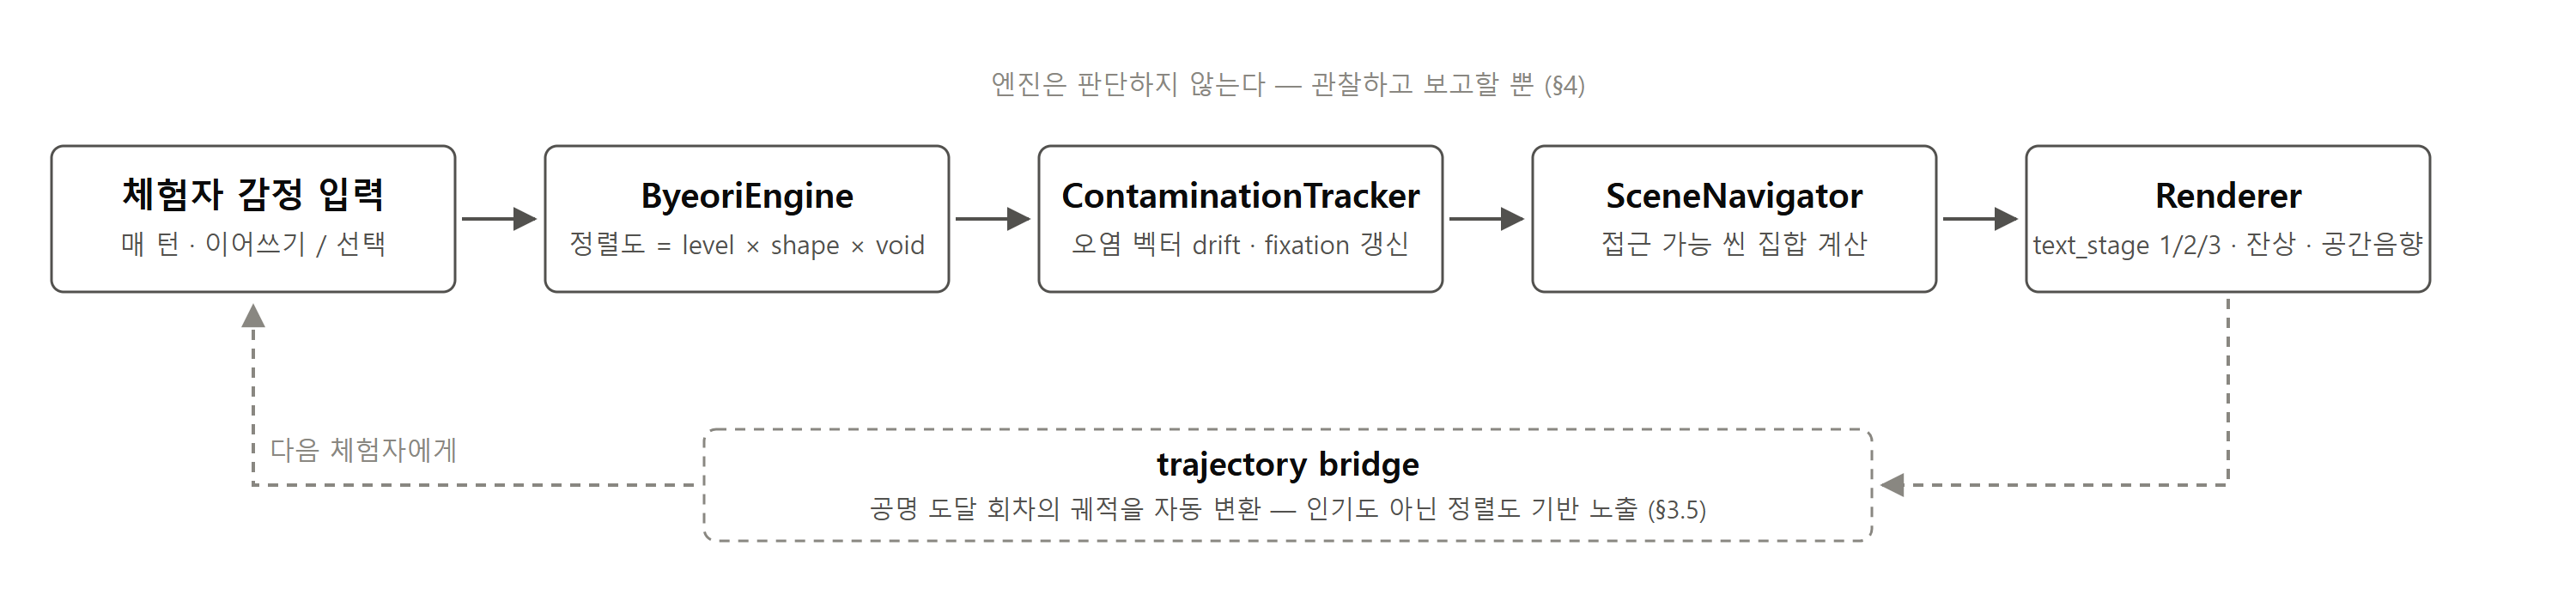
\includegraphics[width=\textwidth]{figures/trackA_fig1_pipeline-260804.png}
\caption{TEM 런타임 파이프라인. 매 턴 체험자 감정 입력이 정렬도(\S4.1)·오염 벡터(\S4.2)·접근 가능 씬 집합(\S3.3) 계산을 거쳐 렌더링으로 이어진다. 공명 도달 회차의 궤적은 trajectory bridge로 자동 변환되어 다음 체험자의 체험에 노출된다(\S3.5).}
\label{fig:pipeline}
\end{figure}

% ════════════════════════════════════════
\section{메트릭}

\subsection{Byeori Engine V4 --- Trajectory Alignment}

별이엔진 V4는 체험자 감정 시퀀스와 작가 원본 감정 시퀀스의 유사도를 실시간으로 산출한다. 정렬도의 정식 정의와 산출 코드는 별도의 기술 명세서(\textit{Byeori Engine Technical Specification --- V4})에 있으며, 그 명세서는 프로덕션 모듈 \texttt{js/core/ByeoriEngine.js} 및 \texttt{js/shared/math.js}와 대조 검증되어 있다. 정렬도는 \textbf{세 인자의 곱}으로 정의된다:
\begin{equation}
\text{alignment} = \operatorname{clamp}_{[0,1]}\big(\, \text{level} \times \text{shape} \times \text{void\_mod} \,\big)
\end{equation}

\begin{itemize}
  \item \textbf{level} --- 방문한 각 씬에서 체험자 감정 벡터와 원본 감정 벡터의 코사인 유사도(\texttt{scene\_score})의 평균. ``장면마다 감정이 얼마나 비슷했는가''의 누적 지표.
  \item \textbf{shape} --- 감정 변화량(delta) 궤적의 형태 유사도. 씬이 3개 이상일 때
  \[ \text{shape} = \max\!\big(0,\ \cos(\operatorname{flatten}(\Delta u),\ \operatorname{flatten}(\Delta o))\big), \]
  그 미만일 때는 중립값 1.0. 원본 궤적은 체험자의 방문 순서대로 재배열된다 --- 어떤 씬을 먼저 여는가가 이미 해석 행위이기 때문이다.
  \item \textbf{void\_mod} --- 체험자가 감정 입력을 회피(VOID)했고 작가는 감정을 드러냈을 때 $\times 0.7$, 그 외 $\times 1.0$.
\end{itemize}

세 인자를 더하지 않고 \textbf{곱한} 것이 이 설계의 요점이다. 선형 결합에서는 한 축이 낮아도 다른 축이 보상할 수 있지만, 곱셈은 그 보상을 구조적으로 막는다. level $= 0$이면 shape가 아무리 높아도 정렬도는 0이 된다. shape가 감정 변화의 \textit{방향}(수준이 아니라 형태)을 비교한다는 점이 TIES 원리의 핵심 이식이다. 두 사람의 감정 수준이 달라도 변화 방향이 유사하면 shape는 높다.

\noindent\textbf{계산 속성.} (1)~\textit{결정론적}: 동일 입력 궤적에 대해 동일 출력, 골든 픽스처로 스냅샷 테스트됨. (2)~\textit{실시간}: 매 턴 $O(8t)$ 이하 비용. (3)~\textit{단조성 불보장}: 단일 턴에서 정렬도가 하락할 수 있음(설계 결정, \S6에서 논의).

\subsection{Contamination Vector --- Drift \& Fixation}

오염 벡터는 체험자 궤적이 원본에서 이탈하는 \textbf{두 가지 분리된 양식}을 측정한다.

\subsubsection{Drift (방향 이탈)}
drift는 \textbf{방향성 누적 이탈}이다. 체험자 궤적의 연속 차분 벡터와 원본 궤적의 연속 차분 벡터가 얼마나 다른 방향을 가리키는지의 누적량:
\begin{equation}
\text{Drift}(U, O) = \frac{1}{t-1} \sum_{i=2}^{t} \left\| (u_i - u_{i-1}) - (o_i - o_{i-1}) \right\|
\end{equation}

\subsubsection{Fixation (단일점 수렴)}
fixation은 \textbf{특정 감정이나 귀인에 과도하게 머무는} 정도이다. TEM 매뉴얼 §8.3은 이를 3-way 복합 신호로 정의한다:
\begin{lstlisting}
signal_sim   = 1  if emotion cosine sim with previous state >= 0.85, else 0
signal_attr  = 1  if attribution repetition ratio of last 3 turns >= 0.8, else 0
signal_expl  = 1  if exploration rate (visited / total scenes) <= 0.3, else 0

Fixation = 0.5 * signal_sim + 0.3 * signal_attr + 0.2 * signal_expl
FIXATED  iff Fixation >= 0.65
\end{lstlisting}
현재 코드는 \texttt{signal\_sim} 한 축만 구현되어 있으며, 전체 복합 신호 구현은 진행 중이다. 본 논문의 \S5 평가는 복합 신호 정의를 기준으로 기술하되, 현 구현과의 격차는 \S6.2에 한계로 명시한다.

\subsubsection{왜 두 축인가 --- 분별력의 동기}
동일 총 이탈량(예: 정렬도 0.4)이라도, \textbf{drift-dominant}한 체험과 \textbf{fixation-dominant}한 체험은 체험적으로 구분된다. 전자는 ``다른 길로 빠지는'' 느낌이고 후자는 ``한 지점에 꽂혀 되풀이되는'' 느낌이다. 두 축을 분리하지 않으면 동일 총량 값으로 뭉뚱그려진다. TEM의 렌더링 결정 --- text\_stage\_2/3 편향 텍스트 생성 조건, NPC 독백 트리거 조건 --- 은 두 축을 독립적으로 참조한다.

\subsection{메트릭의 한계 (선언적으로)}
\begin{enumerate}
  \item \textbf{감정 벡터 부여는 작가 자기보고에 의존한다.} 씬의 \texttt{emotion\_vector}는 작가 혹은 작가+AI 협업으로 할당된다. 외부 rater 혹은 독립 측정과의 수렴 타당성은 확인되지 않았다.
  \item \textbf{체험자 입력은 이산적이다.} 다지선다 혹은 슬라이더 값이며, 연속적 생리 신호(심박, GSR)와 같은 외재 측정이 아니다.
  \item \textbf{Ground truth 부재.} 어떤 궤적이 ``올바른'' 궤적인지에 대한 기준이 없다. 이는 본 메트릭이 \textit{부합}이나 \textit{정확성}이 아니라 \textit{유사도와 이탈 양식}을 측정하도록 설계된 결과이다.
\end{enumerate}

% ════════════════════════════════════════
\section{평가}

\subsection{데이터}
본 논문의 평가는 \textbf{페르소나 시뮬레이션 데이터}로 수행된다. 실제 인간 체험자에 대한 표집 연구는 범위 밖이며 별도 후속 작업에서 다룬다(\S6.3). 다만 공개 알파 테스트에서 수집된 3인 파일럿 관찰을 \S5.5에 예비 보고한다. 페르소나 시뮬레이션은 실제 인간 307{,}313명의 IPIP-NEO-300 Big Five 응답 분포에서 층화 표집한 성격 백본 위에 합성 체험자를 LLM으로 구동하여 생성한다. 본 논문의 데이터셋은 단일 작품이다: \textbf{MM23L ``당신에게''} --- \textbf{193 장면-플레이} (페르소나 15명, 39회차; 2026-07-05 재생성, seed$=$42, 페르소나당 방문 2--4회, 방문당 씬 4--7개를 무작위 순서로).

\noindent\textbf{표기 정정.} v0.4와 ICIDS 2026 제출본은 이 자료를 ``193 plays''라고 적었다. 정확한 단위는 \textbf{씬 하나에 대한 응답 하나}(장면-플레이)이며, 회차(한 페르소나의 한 방문)로 세면 \textbf{39회차}다. 페르소나별 회차 수는 2회가 7명, 3회가 7명, 4회가 1명이고, 페르소나별 장면-플레이 수는 8--20건이다. 장면-플레이는 페르소나 안에 묶여 있어 서로 독립이 아니므로, \S5.3의 상관은 193건이 아니라 페르소나 15명의 평균 위에서 계산한다.

각 플레이는 씬별 emotion\_vector, alignment, mismatch\_type, inner\_reason을 기록한다. 정렬도는 두 가지로 측정된다: \textbf{직접 계산(objective)} $=$ 페르소나 감정 분포와 원본 감정 분포의 코사인 유사도(본 논문의 1차 측정), \textbf{자기보고(self-report)} $=$ LLM이 스스로 매긴 점수(순환적이므로 비교 신호로만 사용).

\noindent\textbf{데이터 계보 각주.} 2026년 4월의 최초 생성분(MM23L 193 + E-004 100 $=$ 293 plays)은 이후 DB 재적재 과정에서 유실되었고, E-004는 작품 자체가 DB에서 제거되어 재생성이 불가하다. 본 논문의 모든 수치는 2026-07-05 재생성된 MM23L 193 장면-플레이 기준이다. 표집 단계는 결정론적(seed$=$42)이라 15개 페르소나의 성격 점수는 4월분과 동일하나, LLM 생성 단계는 비결정론적이므로 4월분과의 직접 비교는 하지 않는다.

\subsection{가설}
\textbf{H1. 성격→정렬도 분별력.} 페르소나 Big Five 프로파일(특히 Agreeableness, Openness, Extraversion)에 따라 최종 정렬도 분포가 이론적으로 예측되는 방향으로 구분된다.

\textbf{H2. 극단 페르소나의 분포 꼬리 형성.} 층 설계에서 ``시스템을 거스르도록'' 겨냥한 극단 페르소나는 정렬도 분포의 중앙이 아니라 꼬리를 형성한다.

\textbf{H3. 계측기의 분포 특성.} 시뮬레이션 정렬도 분포가 붕괴(전원 공명 또는 전원 불일치)하지 않고 스펙트럼을 재현하며, 계측기 내부 분별력을 가진다.

\subsection{결과}

\textbf{분포 특성 (표~\ref{tab:dist}).} 직접 계산 정렬도는 평균 0.809, 표준편차 0.149, 범위 0.254--0.986이었다. 어긋남(mismatch) 발생률은 97.4\%였고, 어긋남 유형은 target\_displacement가 159/193(82.4\%)으로 압도적이었다. 자기보고 정렬도는 세 값(0.72/0.62/0.52)에 71.0\%가 몰려 실효 범위가 0.42--0.82로 잘렸다 --- 자기보고 점수는 양자화되어 연속 측정도구로 부적격이며, 정렬도는 감정 분포에서 직접 계산해야 함이 실측으로 확인된다.

\begin{table}[H]
\centering
\caption{193 장면-플레이의 정렬도 분포 특성}
\label{tab:dist}
\begin{tabular}{l l}
\toprule
\textbf{특성} & \textbf{관측값 (직접 계산, $n=193$)} \\
\midrule
정렬도 평균 & 0.809 \\
정렬도 표준편차 & 0.149 \\
정렬도 범위 & 0.254 -- 0.986 \\
어긋남 발생률 & 97.4\% \\
지배적 어긋남 유형 & target\_displacement (82.4\%) \\
\bottomrule
\end{tabular}
\end{table}

\textbf{H1 --- 성격과 정렬도의 상관 (Pearson $r$, $n=15$ 페르소나).} 개방성(O)·친화성(A)·외향성(E)이 페르소나 평균 정렬도와 양의 상관을 보였다(표~\ref{tab:corr}). 보정 전 양측 $p$는 각각 .011, .021, .034다. 그러나 다섯 특질을 함께 검정했으므로 Holm 보정을 하면 .056, .083, .102가 되어 \textbf{어느 것도 .05 문턱을 넘지 못한다.} 95\% 신뢰구간(Fisher $z$)도 넓어서 하한이 0에 가깝다(개방성 0.18--0.87). 페르소나를 다시 뽑는 부트스트랩(1만 회) 구간도 비슷하며(O 0.05--0.86, A 0.12--0.85, E 0.22--0.80), 순위 상관(Spearman)은 O 0.529, A 0.490, E 0.552로 방향이 같다.

따라서 H1에 대해 이 자료가 말할 수 있는 것은 ``세 특질에서 방향이 일관된 양의 연관이 관찰되었다''까지다. $n=15$에서 이것을 확증으로 읽을 수 없으며, v0.4의 ``유의하게 예측했다''는 표현은 이 판에서 거둔다. 신경증(N)·성실성(C)에서는 연관이 관찰되지 않았다. 예측 밖 관찰로, 세 특질 가운데 개방성의 계수가 가장 컸다($r=0.634$). 계산 절차는 부록~\ref{app:stats}에 있다.

\begin{table}[H]
\centering
\caption{성격 특질과 직접 계산 정렬도(페르소나 평균)의 상관, $n=15$. 신뢰구간은 Fisher $z$, 보정은 다섯 특질에 대한 Holm 절차}
\label{tab:corr}
\small
\begin{tabular}{l c c c c}
\toprule
\textbf{Big Five 축} & \textbf{$r$} & \textbf{95\% 신뢰구간} & \textbf{$p$ (보정 전)} & \textbf{$p$ (Holm)} \\
\midrule
Openness (O) & 0.634 & [0.18, 0.87] & .011 & .056 \\
Agreeableness (A) & 0.590 & [0.11, 0.85] & .021 & .083 \\
Extraversion (E) & 0.549 & [0.05, 0.83] & .034 & .102 \\
Conscientiousness (C) & 0.192 & [$-$0.36, 0.64] & .494 & .987 \\
Neuroticism (N) & 0.131 & [$-$0.41, 0.60] & .642 & .987 \\
\bottomrule
\end{tabular}
\end{table}

\textbf{H2 --- 극단 페르소나 (절반 지지).} 냉소적 해체자 p08(low\_A\_low\_C)은 15명 중 최하위(0.638)로 분포의 낮은 꼬리를 만들며 분리에 성공했다. 그러나 그늘을 이해 못 하도록 겨냥한 극단 낙관형 p15는 7위(0.840) 중위권에 머물렀다. \textbf{부정 극단은 시뮬레이션되나 ``공감 실패''는 시뮬레이션되지 않는다} --- 이 비대칭이 계측기의 한계다. 순위 상단은 p09(0.917), p06 공감적 경청자(0.876)로 이론과 정합했다.

\textbf{H3 --- 과공명 천장 편향 (계측기 한계로 규정).} 15개 페르소나 전원이 평균 0.64 이상으로 떠 있고, 인간 독자에게 기대되는 낮은 꼬리($< 0.25$)가 없었다. LLM 시뮬레이션 독자는 \textbf{과공명(over-resonance)}한다. 성격 축을 실제 분포로 표집해도 감정 반응 생성 단계에서 상향 편향이 되살아난다. 따라서 이 계측기는 \textbf{상대 비교에서는 유효하지만 절대 분포에서는 천장 편향}을 보인다. 우리는 이것을 도구의 실패로 보지 않고 측정된 경계로 읽는다(\S6.2). 단, 이 편향의 원인을 LLM의 성향 하나로 돌릴 수는 없다. 시뮬레이션 프롬프트는 씬의 원본 감정 분포를 ``참고용, 복사 금지''라는 말과 함께 독자에게 보여 주며(부록~\ref{app:sim}), 직접 계산 정렬도는 바로 그 분포와의 코사인이다. 천장 편향의 일부는 이 노출에서 왔을 수 있고, 두 원인은 원본 감정을 가린 재실행으로만 갈라낼 수 있다. 파일럿 인간 관찰(\S5.5)은 이 경계와 정합하는 첫 실측 신호를 준다 --- 인간 장면-플레이의 14.3\%가 0.25 아래로 내려간 반면 시뮬레이션은 0건이다.

\subsection{질적 예시 --- 페르소나 p08 (냉소적 해체자)}
정량 분석을 보완하기 위해, 낮은 꼬리를 만든 유일한 페르소나 p08(low\_A\_low\_C; 실측 $N=86.3$, $A=25.0$, $C=29.3$, 직접 계산 정렬도 최하위 0.638)의 10장면 궤적을 엔드투엔드로 읽는다. 이 트레이스는 그 꼬리가 잡음이 아니라 \textbf{성격 표집 점수 → 전기 → 씬 반응}의 심리적으로 일관된 사슬임을 보인다 --- 표집된 고신경증·저친화 점수가 임종 전화를 회피한 전기로 확장되고, 그 전기가 매 씬에서 자기 어머니를 소환하는 반응으로 이어진다. 어느 단계에도 성격 딱지 없이, 서로 다른 모델이 생성했음에도 예측과 행동이 맞아떨어진다.

\subsection{파일럿 인간 관찰 --- 3인 21 장면-플레이}

\S5.4까지의 평가는 시뮬레이션 내부 타당성에 한정된다. 본 절은 2026년 8월 공개 알파 테스트에서 수집된 실제 인간 체험자 3인의 완주 3회차(21 장면-플레이)를 예비 관찰로 보고한다. 이는 표집된 연구가 아니라 파일럿 관찰이며(\S5.6의 한계 그대로), \S6.3에 예고된 인간 체험자 연구($N=30$--$50$)의 사전 신호로만 읽어야 한다.

측정은 \S5.1과 동일하다 --- 정렬도는 체험자 감정 분포와 씬 원본 감정 분포의 코사인 유사도로 직접 계산되며, 라이브 시스템이 저장한 값과 오프라인 재계산 값이 21건 전부 일치함을 확인했다(상관 1.000, 평균절대오차 0.000). 인간 체험자의 감정 분포는 자유 서술 텍스트에서 LLM 추출로 얻어지고, 페르소나의 감정 분포는 역할 수행 LLM이 직접 산출한다 --- 두 경로 모두 LLM을 경유하나 입력 양식이 다르다는 점은 아래 한계에 명시한다.

\begin{table}[H]
\centering
\caption{정렬도 분포 --- 파일럿 인간 대 페르소나 시뮬레이션 (동일 공식)}
\label{tab:pilot}
\begin{tabular}{l l l}
\toprule
 & \textbf{인간 파일럿 ($n=21$)} & \textbf{페르소나 시뮬 ($n=193$)} \\
\midrule
평균 & 0.517 & 0.809 \\
표준편차 & 0.211 & 0.149 \\
범위 & 0.114 -- 0.781 & 0.254 -- 0.986 \\
$< 0.42$ 비율 & 28.6\% & 3.1\% \\
$< 0.25$ 비율 & \textbf{14.3\%} & \textbf{0.0\%} \\
\bottomrule
\end{tabular}
\end{table}

\begin{figure}[H]
\centering
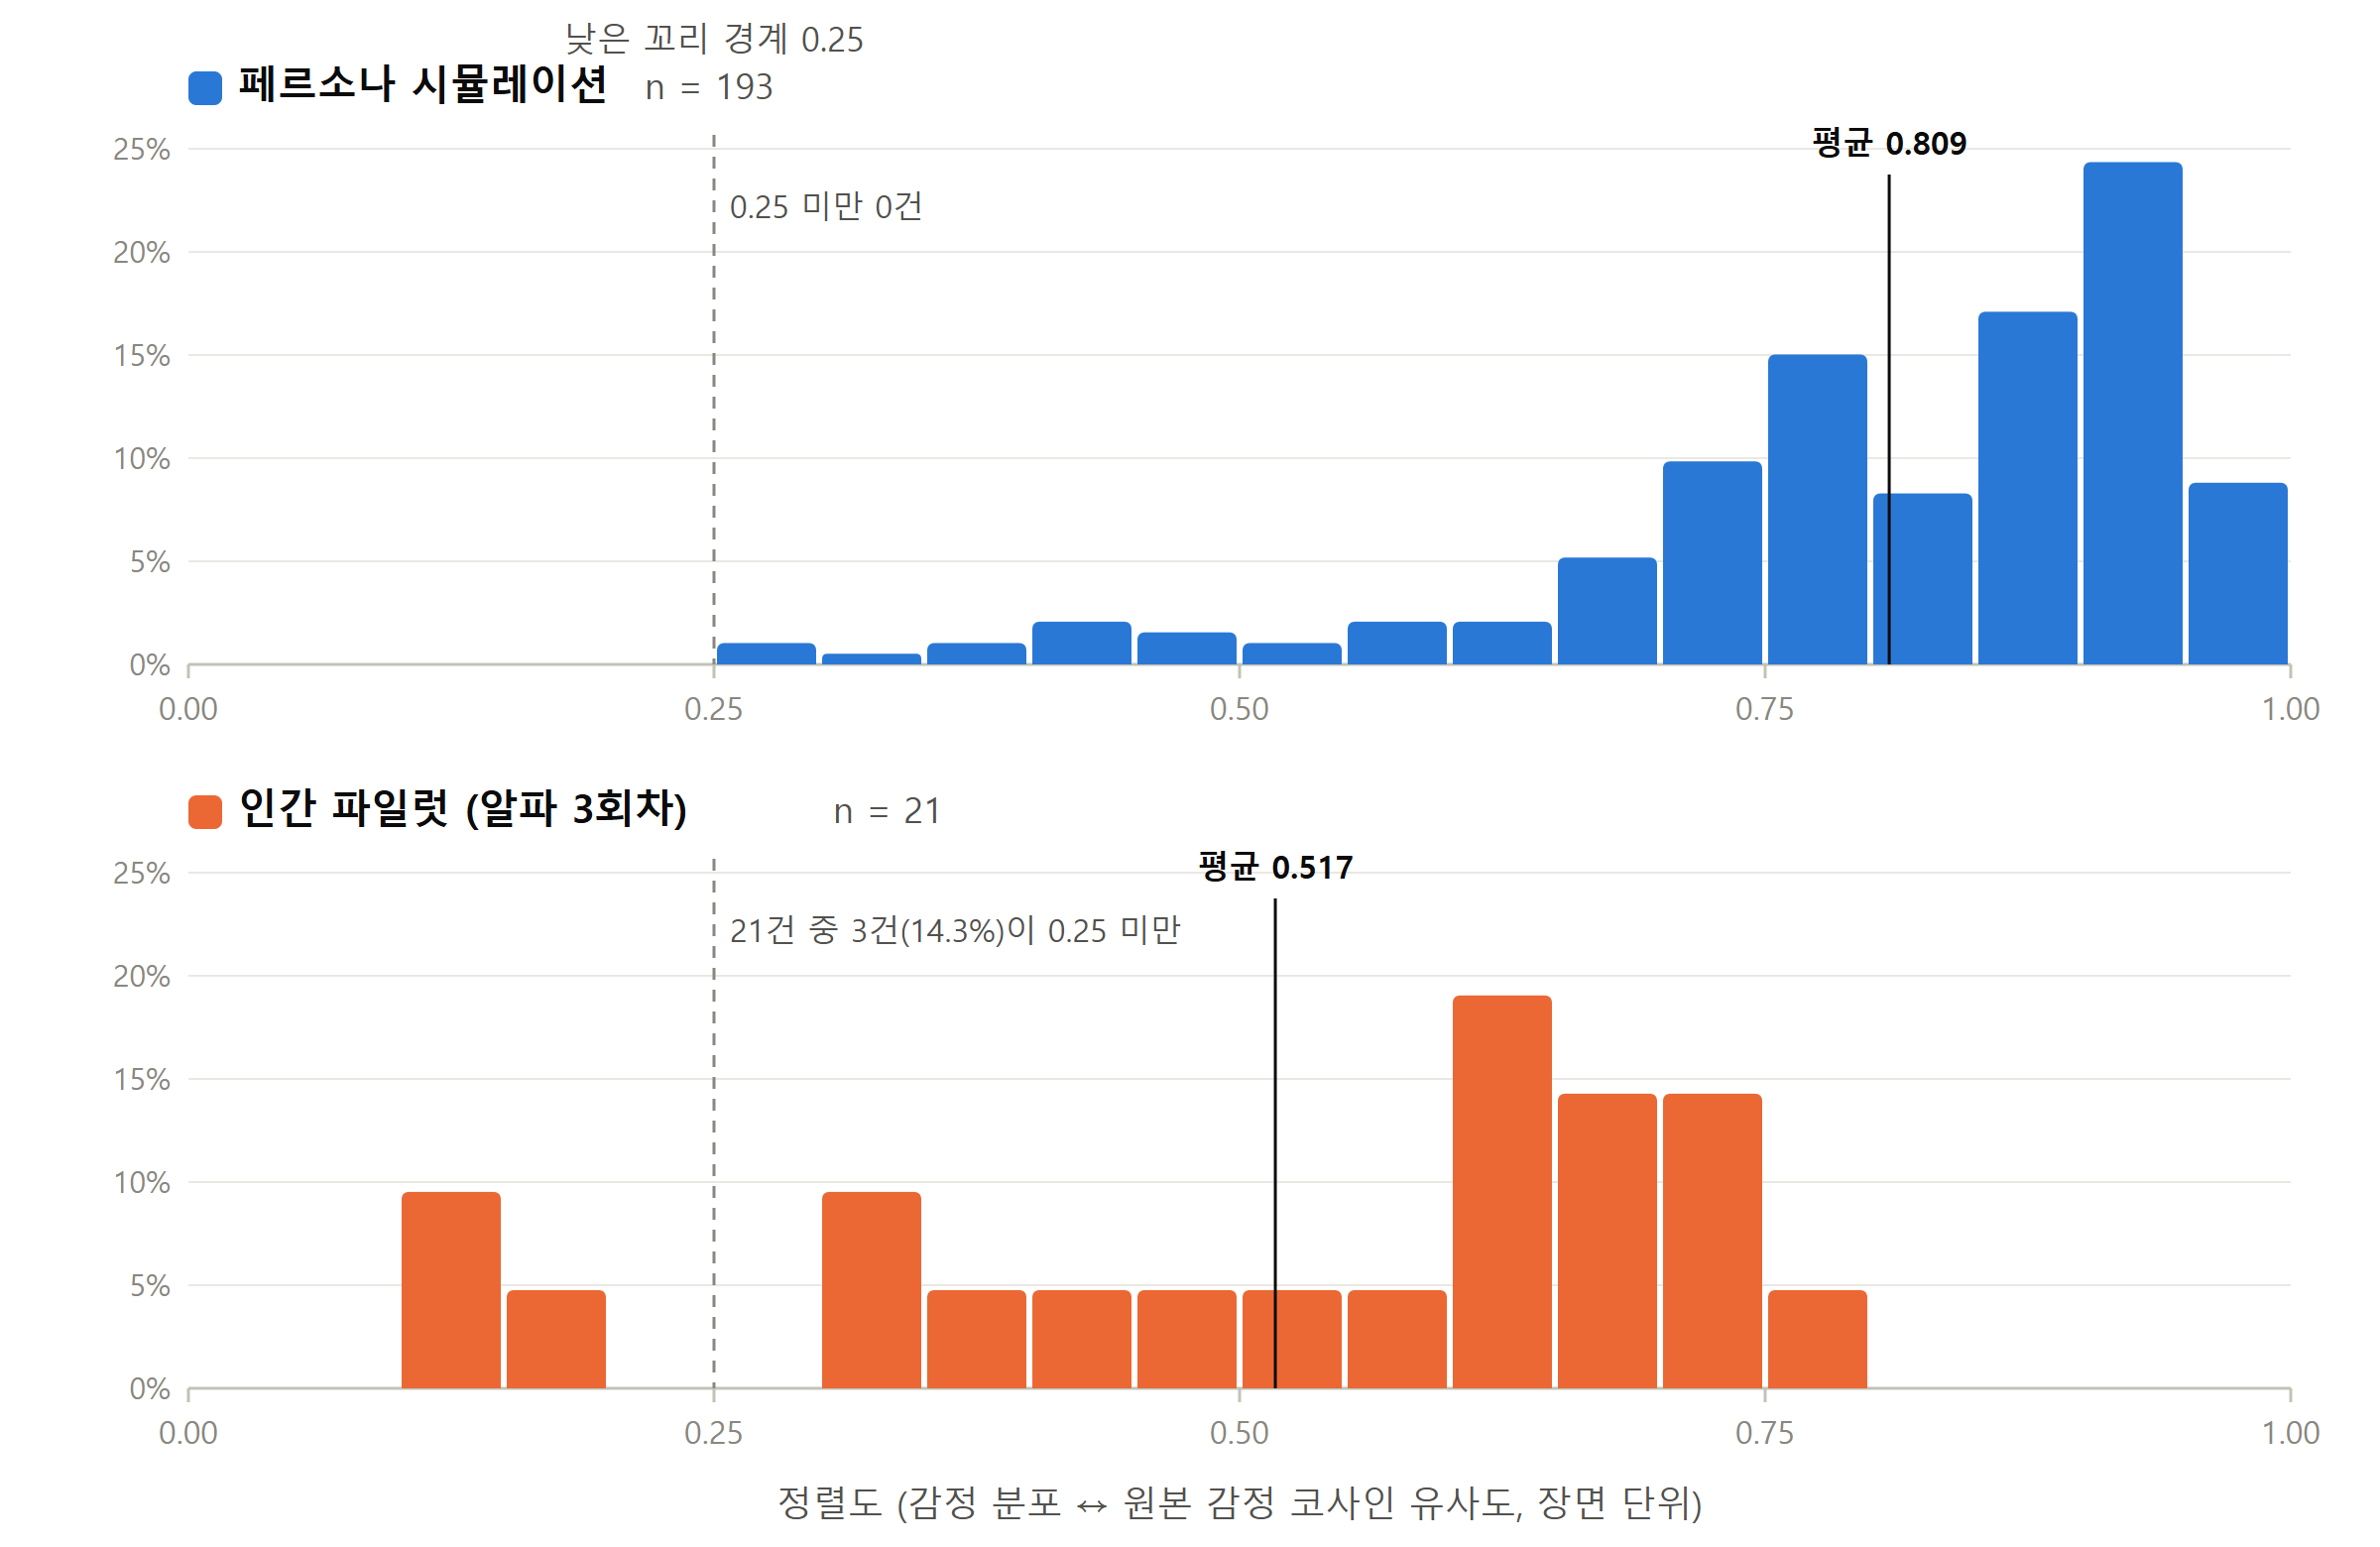
\includegraphics[width=\textwidth]{figures/trackA_fig2_dist-260804.png}
\caption{정렬도 분포 대조(장면 단위, 동일 공식). 위: 페르소나 시뮬레이션($n=193$) --- 0.25 미만 0건. 아래: 인간 파일럿($n=21$) --- 14.3\%가 0.25 미만. 시뮬레이션이 재현하지 못한 낮은 꼬리가 인간 분포에 실재한다.}
\label{fig:pilotdist}
\end{figure}

세 가지가 관찰된다.

\textbf{첫째, 낮은 꼬리의 실재 (그림~\ref{fig:pilotdist}).} \S5.3(H3)은 시뮬레이션 분포에 ``인간 독자에게 기대되는 낮은 꼬리($<0.25$)가 없다''고 보고했고, 그 기대는 당시 가정이었다. 파일럿에서 인간 장면-플레이의 14.3\%가 0.25 아래로 내려갔다(최저 0.114). 시뮬레이션 193건 중 0.25 미만은 0건이다. 과공명 천장 편향이라는 계측기 경계 규정(\S5.3)과 방향이 정합하는 첫 인간 신호다.

\textbf{둘째, 분산 폭.} 인간 파일럿의 표준편차(0.211)는 시뮬레이션(0.149)의 1.4배다. 회차 평균도 0.633 / 0.522 / 0.456으로 세 체험자가 서로 다른 높이에 앉는다. LLM 페르소나가 성격 축을 실제 분포로 표집해도 재현하지 못한 흩어짐이 인간 3인에서 이미 나타난다.

\textbf{셋째, 경로 분기의 실측.} \S3.3의 설계 --- 분기 그래프 없이 감정 상태가 경로를 결정한다 --- 가 처음으로 인간 궤적에서 관찰되었다. 세 체험자의 씬 시퀀스는 그림~\ref{fig:paths}와 같다.

\begin{figure}[H]
\centering
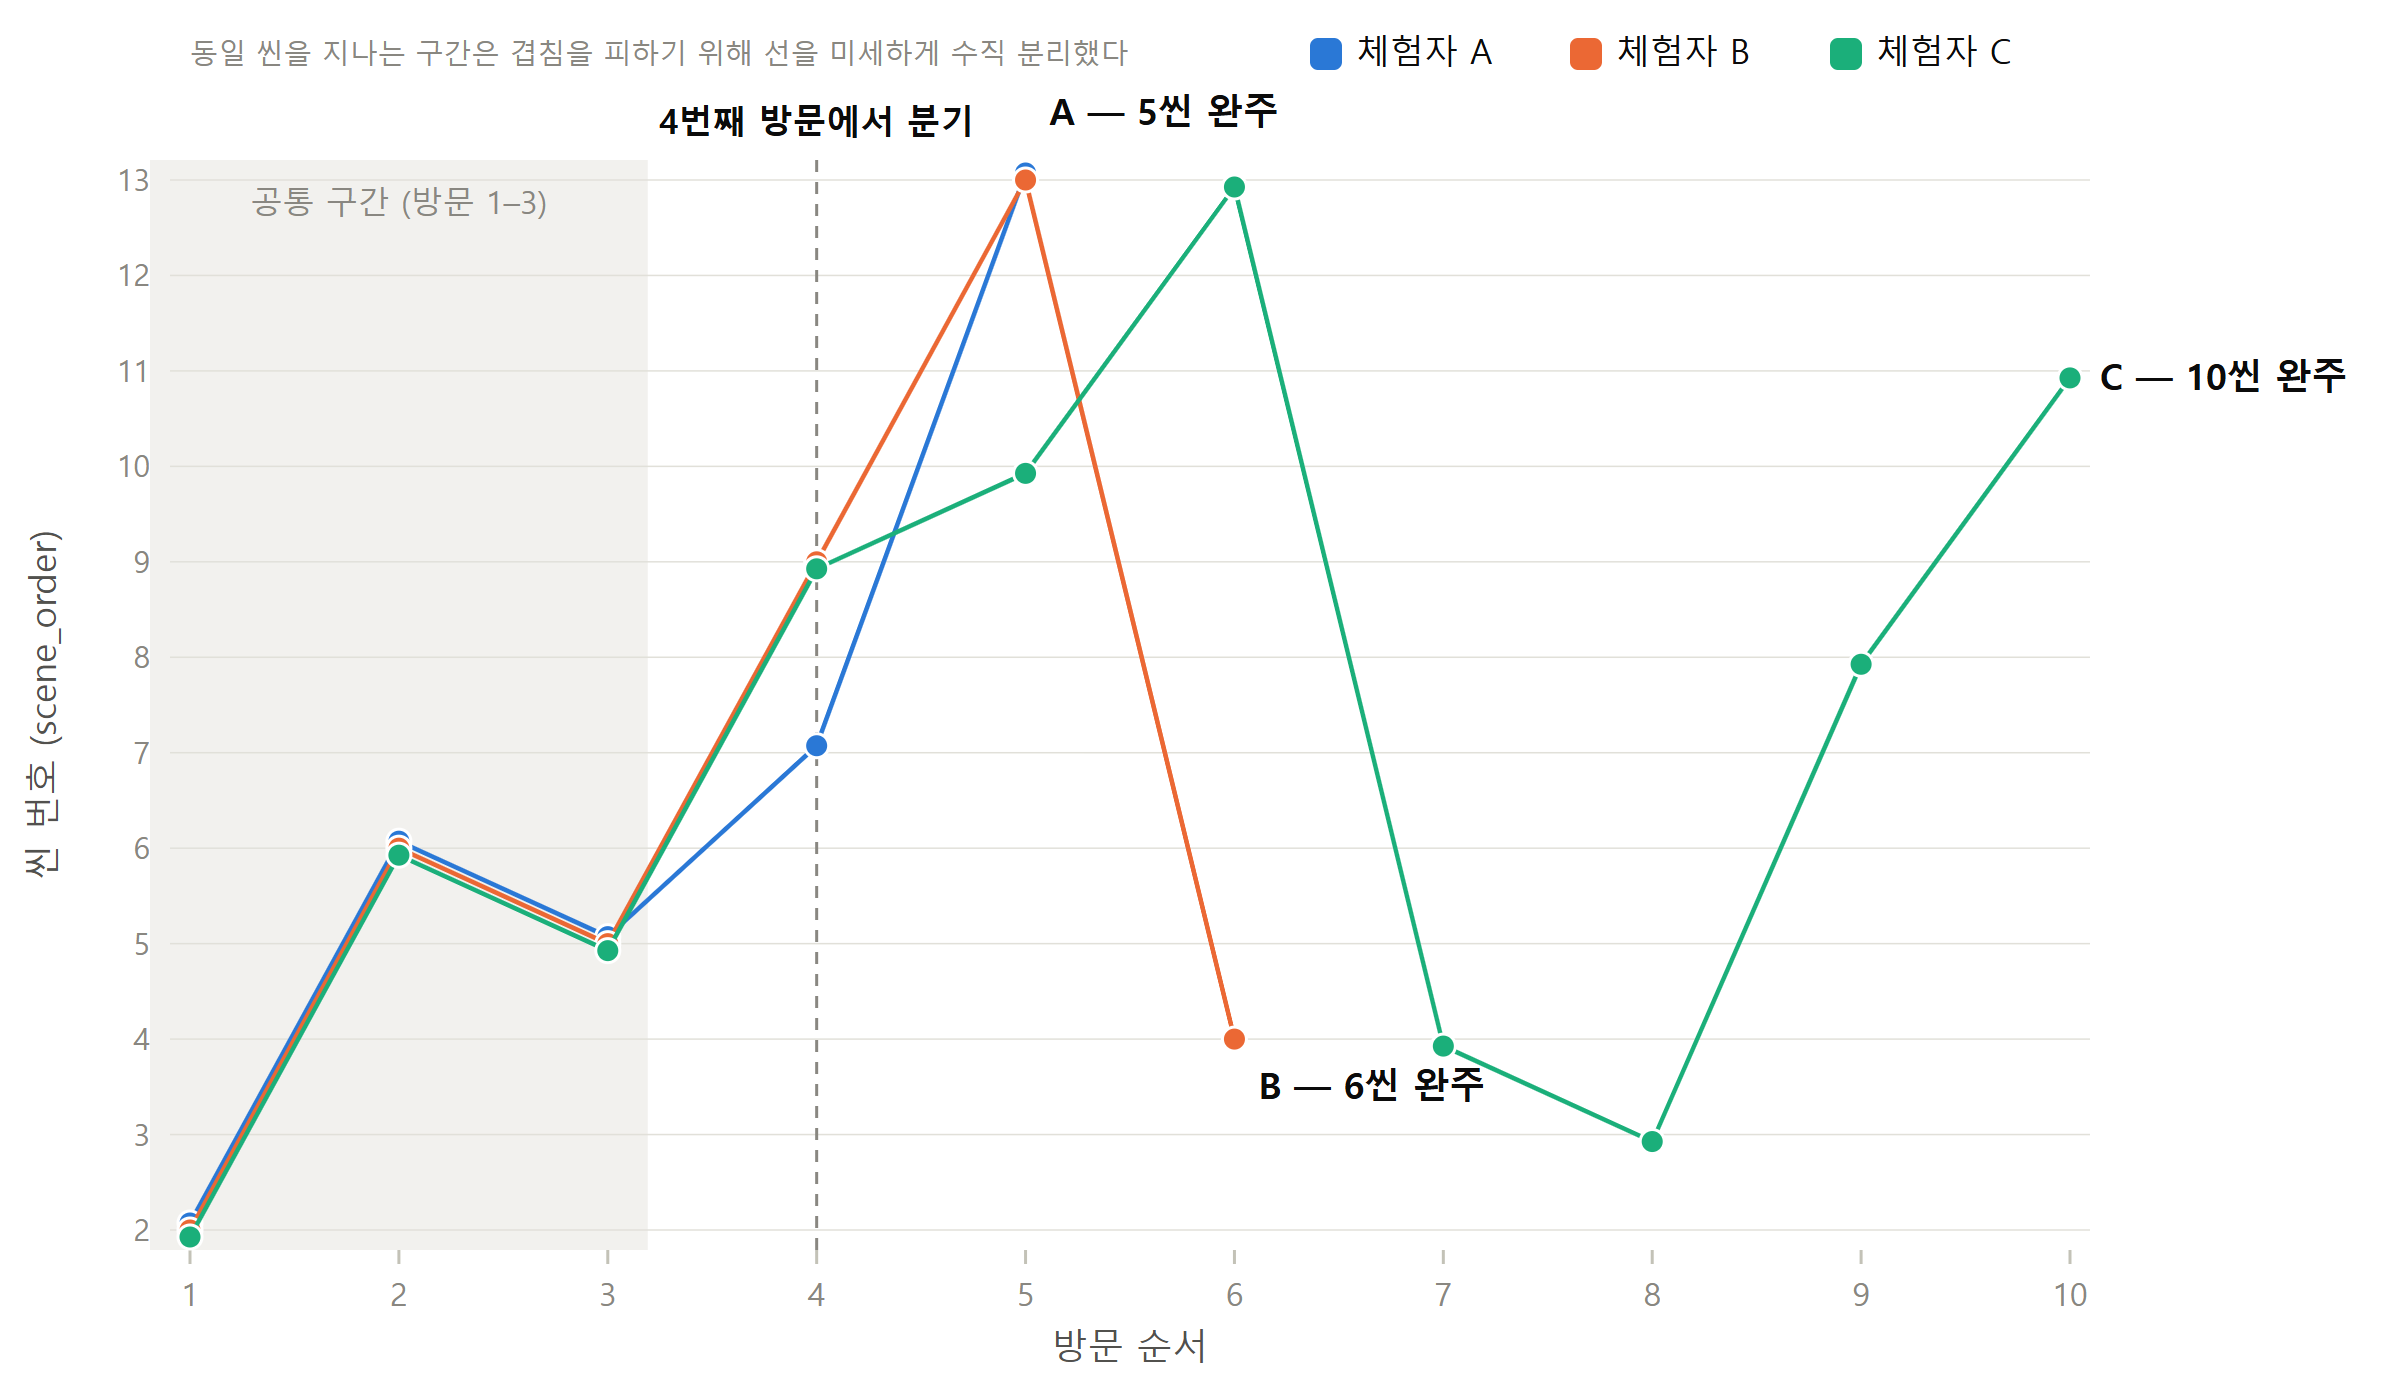
\includegraphics[width=\textwidth]{figures/trackA_fig3_paths-260804.png}
\caption{세 체험자의 씬 시퀀스(scene\_order). 앞 세 방문은 동일하고, 네 번째 방문에서 분기가 시작된다. 동일 씬을 지나는 구간은 겹침을 피하기 위해 선을 미세하게 수직 분리했다.}
\label{fig:paths}
\end{figure}

분기는 네 번째 장면에서 시작된다. 앞 세 장면이 동일한 것은 결함이 아니라 설계의 귀결로 읽힌다 --- 정렬도의 shape 인자는 3개 장면 이상에서만 활성화되므로(\S4.1), 궤적 기반 접근이 개인화되기까지 워밍업 구간이 존재한다. 이 구간의 길이가 shape 활성 시점과 일치하는지는 표본이 쌓여야 분리 검증할 수 있다.

\textbf{이 관찰이 주장하지 않는 것.} (1) 인간 파일럿은 시뮬레이션과 \textbf{다른 작품}에서 수집되었다(시뮬레이션 $=$ MM23L, 파일럿 $=$ 별도 작품). 평균 격차 0.292의 일부는 작품 차이일 수 있으며, 동일 작품 인간 데이터가 쌓이기 전까지 이 비교는 분포 형태(꼬리·분산)의 대조로만 유효하다. (2) 어긋남 유형(mismatch\_type)은 두 집단의 분류기가 달라 비교에서 제외했다. (3) $n=3$은 편의 표본이며 IRB 심의를 거치지 않았다 --- 통계적 주장이 아니라 방향 신호다.

\subsection{평가하지 않는 것}
본 평가는 다음을 주장하지 않는다: \textbf{외적 타당성} --- 페르소나 시뮬은 LLM의 감정 모델을 경유하므로, 이 결과는 실제 인간 체험자의 행동을 담보하지 않는다(\S5.5의 파일럿은 방향 신호일 뿐 이 한계를 해제하지 않는다). 페르소나 결과는 \textbf{메트릭의 계산적 일관성과 내부 분별력}의 증거이다. \textbf{인지심리학적 주장} --- 본 메트릭은 기억 변형의 인지적 메커니즘에 대한 어떤 주장도 하지 않는다.

\subsection{제목이 약속한 것과 실제로 잰 것}

ICIDS 2026 심사는 ``제목은 궤적과 오염인데, 평가한 숫자는 장면별 순간 유사도뿐''이라고 지적했다. 맞는 지적이며, 숨기지 않고 표~\ref{tab:gap}에 적는다.

\begin{table}[H]
\centering
\caption{구성 요소별 --- 구현되었는가, 수치로 평가되었는가}
\label{tab:gap}
\small
\begin{tabular}{p{5.4cm} c p{6.6cm}}
\toprule
\textbf{구성 요소} & \textbf{구현} & \textbf{수치로 평가했는가} \\
\midrule
level (장면별 코사인) & 완료 & \textbf{예} --- \S5.3, \S5.5 \\
shape (변화량 궤적의 형태) & 완료 & \textbf{아니오} \\
오염 벡터 2축 (drift, fixation) & 완료 & \textbf{아니오} \\
공명 사건 & 완료 & 희소성만 측정 (사람 29턴 중 0회) \\
trajectory bridge 릴레이 & 완료 & \textbf{아니오} \\
궤적 이력이 순간 유사도보다 나은가 (떼어내기 비교) & --- & \textbf{아니오}. 관련 후보 식 하나는 별도의 사전 등록 백테스트(2026-11-07)에서 기준선을 넘지 못했다 \\
\bottomrule
\end{tabular}
\end{table}

shape가 평가되지 못한 이유는 자료의 구조에 있다. 페르소나 시뮬레이션은 씬을 무작위 순서로 하나씩, 호출마다 따로 읽힌다(부록~\ref{app:sim}). 직접 계산 정렬도는 씬 하나에서의 코사인이고, 변화량 궤적을 요구하는 shape 인자는 이 자료에서 계산되지 않는다. 인간 파일럿의 표~\ref{tab:pilot}도 같은 장면별 코사인이다.

따라서 \S5의 수치가 뒷받침하는 것은 \textbf{level 성분이 독자에 따라 갈린다}는 데까지다. ``궤적''과 ``오염''이라는 말은 이 논문에서 설계와 구현을 가리키며, 그 타당성의 수치 증거는 아직 없다.

% ════════════════════════════════════════
\section{논의 및 한계}

\subsection{기여의 범위 재확인}
본 논문은 세 가지를 기여한다: (1) 감정 궤적을 일차 차원으로 두는 작동 시스템, (2) 두 가지 분리 메트릭(alignment, drift/fixation)의 정의와 구현, (3) 페르소나 시뮬로 시범 평가한 level 성분의 분별력(\S5.7의 범위 안에서). 본 논문은 다음을 주장하지 \textbf{않는다}: 기억 변형의 인지심리학적 메커니즘, 인간 체험자에 대한 외적 타당성, 어떤 궤적이 ``올바른'' 궤적인지에 대한 규범적 판단.

\subsection{한계}
\begin{itemize}
  \item \textbf{감정 벡터 ground truth 부재}: 씬 감정 벡터가 작가 자기보고 → 복수 작가 교차 검증 혹은 독립 rater 필요.
  \item \textbf{fixation 복합 신호 부분 구현}: \S4.2.2의 3-way 복합 신호 중 현 코드는 \texttt{signal\_sim} 한 축만 구현. 그 전까지 fixation 결과는 단축 신호 기준임을 명시한다.
  \item \textbf{LLM 기반 페르소나의 편향}: LLM의 감정 모델 편향이 결과에 유입 → 복수 LLM 비교 혹은 인간 보정 필요.
  \item \textbf{원본 감정의 프롬프트 노출}: 시뮬레이션 독자는 씬의 원본 감정 분포를 본 채로 응답했다(부록~\ref{app:sim}). 직접 계산 정렬도의 높은 평균이 이 노출과 섞여 있다.
  \item \textbf{같은 모델의 역할극}: 15 페르소나는 한 모델이 연기한 것이므로 독립된 독자 15명의 표본이 아니다.
  \item \textbf{통계}: $n=15$의 상관 다섯 개는 다중비교 보정 뒤 .05 문턱을 넘지 못한다(\S5.3). 평가된 것은 level 성분뿐이다(\S5.7).
  \item \textbf{공명 판정의 임계값 민감도}: 현재 공명 기준은 heuristic이며 민감도 분석 부재.
  \item \textbf{명시적 분기 부재의 한계}: 일부 서사적 순간(작가가 의도한 결정적 갈림길)은 감정 거리만으로 유도가 어려움. 향후 ``작가 포트'' 모델로 보완 예정.
\end{itemize}

\subsection{향후 작업}
\begin{itemize}
  \item \textbf{인간 체험자 연구 (IRB + $N=30$--$50$)}: 페르소나 결과의 외적 타당성 검증. \S5.5 파일럿이 시사한 두 대조 --- 낮은 꼬리의 실재, 1.4배 분산 --- 의 재현이 1차 확인 대상이며, 동일 작품 수집으로 작품 교란을 제거한다.
  \item \textbf{Trajectory bridge 품질 연구}: 자동 승인된 궤적 브릿지가 다음 체험자에게 미치는 영향 --- 노출 이후 alignment / drift / fixation 변화 추적.
  \item \textbf{원본 감정을 가린 시뮬레이션 재실행}: 프롬프트에서 원본 감정 분포를 뺀 조건과 넣은 조건을 나란히 돌려, 천장 편향 가운데 노출 몫을 갈라낸다.
  \item \textbf{떼어내기 비교}: 순간 유사도만 쓴 점수와 궤적 이력을 쓴 점수를 같은 자료에서 나란히 놓아, shape 인자가 무엇을 더하는지 잰다(\S5.7).
  \item \textbf{복수 작품 교차 검증}: 현재 MM23L 단일 작품. target\_displacement 82.4\% 과점이 작품 주제(죽은 이에게 쓰는 편지)의 유도인지 LLM 범주 편향인지는 주제가 다른 작품에서만 분리 가능하다.
\end{itemize}

% ════════════════════════════════════════
\section{윤리 고려}
체험자 감정 입력은 민감 데이터이다. TEM은 다음 방식으로 대응한다. \textbf{명시적 동의} --- record 단계 confession 화면에서 자신의 기억 조각이 다음 체험자에게 노출될 수 있음에 대한 동의 수집(\texttt{consentLine}). \textbf{PII 필터} --- 잔상(afterimage)에 개인 식별 정보가 포함되지 않도록 17종 케이스 필터 적용. \textbf{안전 설계} --- trigger word 감지 시 즉시 차단이 아닌 $n$회차 에스컬레이션, 시제 감지 기반 판단. \textbf{철회 가능성} --- 사용자 동의 철회 페이지(구현 중). 궤적 브릿지는 \texttt{source\_run\_id}로 역추적 가능하나 표시되지는 않으며, 노출 시 작성자 식별자는 렌더링되지 않는다. record 단계의 동의 문구는 ``이 기억의 조각이 누군가의 장면 끝에 떠올라도 좋다.''이다(영문판: ``Let a fragment of this memory rise in someone else's scene.'').

\subsection*{참가자와 동의}

ICIDS 2026 심사는 ``심의가 없다고 쓰고도 동의 절차를 쓰지 않았다''고 지적했다. 있는 대로 적는다.
\begin{itemize}
  \item 본 연구는 기관 소속 없는 독립 연구이며 기관 심의(IRB)를 거치지 않았다.
  \item \S5.5의 3인 파일럿은 2026년 8월 공개 알파에서 모였다. 알파 설문에서 동의를 받았다. \blank{동의 문구 원문 · 철회 절차 · 익명 처리 방식}
  \item 페르소나 시뮬레이션(\S5.1--5.4)에는 인간 참가자가 없다. 성격 점수는 공개 데이터셋(IPIP-NEO-300 응답, 부록~\ref{app:sim})에서 표집했고, 표집된 행에서 프롬프트로 넘어가는 것은 다섯 성격 점수와 국가·나이·성별뿐이다.
  \item 다음 수집(목표 30명, 동일 작품)은 동의서·철회 절차·익명 처리 문서를 \textbf{수집 전에} 갖춘다. 그 문서가 생기기 전에는 사람 자료를 새로 모으지 않는다.
\end{itemize}

% ════════════════════════════════════════
\section{결론}
상호작용 서사는 체험자마다 다른 경험을 약속해 왔지만, 그 \textbf{다름이 감정의 차원에서 무엇인지}를 말하는 도구는 드물었다. 본 논문은 (1) 감정 궤적을 일차 차원으로 두는 작동 시스템 \textit{The Etched Mutation}, (2) 궤적 형태의 실시간 유사도 측정 \textit{Byeori Engine V4 alignment}, (3) 궤적 이탈의 두 분리 양식 \textit{drift / fixation}, (4) 공명 도달자 궤적의 자동 해석화 \textit{trajectory bridge}를 제시하였으며, 페르소나 시뮬 193 장면-플레이(39회차)로 정렬도의 level 성분을 시범 평가하였다 --- 성격 특질과 정렬도 사이의 양의 연관($r=0.55$--$0.63$, $n=15$, 다중비교 보정 뒤에는 유의 문턱 미달)과, LLM 시뮬레이션 독자의 과공명 천장 편향이라는 계측기의 경계를 함께 보고하였다. shape 성분과 오염 벡터의 수치 평가는 남은 일이다(\S5.7). 공개 알파의 3인 파일럿 인간 관찰은 이 경계의 방향을 실측으로 뒷받침했다 --- 시뮬레이션이 재현하지 못한 낮은 꼬리와 넓은 분산이 인간 분포에 실재했으며, 세 체험자는 분기 그래프 없이 서로 다른 씬 시퀀스를 밟았다.

본 논문이 남기는 것은 거대 이론의 증명이 아니라, 손에 잡히는 \textbf{측정 장치와 체험 시스템}이다. 기억이 변형되며 전파된다는 관찰은 Bartlett 이래 두껍게 쌓여 왔다. 본 논문은 그 변형의 \textbf{양상을 측정 가능한 양으로 분해}하고, 그 양이 흐르는 \textbf{체험 환경을 실제로 구축}했다. 작더라도 하나의 새로운 좌표를 보탠다.

% ════════════════════════════════════════
\appendix
\section{재현 세부}
\label{app:repro}

ICIDS 2026 심사는 엔진 상수, LLM 모델과 프롬프트, 페르소나 구성이 빠져 있다고 지적했다. 아래 값은 전부 저장소의 코드에서 옮겨 적은 것이며(2026-11-20 기준), 괄호 안은 그 값이 있는 파일이다.

\subsection{엔진 상수}
\label{app:engine}

\begin{table}[H]
\centering
\caption{별이엔진 V4와 접근 계산의 상수}
\small
\begin{tabular}{p{4.6cm} p{9.6cm}}
\toprule
\textbf{항목} & \textbf{값} \\
\midrule
정렬도 & $\operatorname{clamp}_{[0,1]}(\text{level}\times\text{shape}\times\text{void\_mod})$ \\
shape 활성 조건 & 방문 씬 3개 이상. 그 전에는 1.0 \\
void\_mod & 체험자만 감정을 비웠을 때 0.7, 그 외 1.0 \\
등급 (bucket) & HIGH $\geq 0.50$ · LOW $< 0.10$ · 그 사이 MID \\
등급 히스테리시스 & 직전이 HIGH면 0.40 이상에서 HIGH 유지 · 직전이 LOW면 0.15 이하에서 LOW 유지 \\
FIXATED & 최근 감정 벡터 3개의 쌍별 코사인 평균 $\geq 0.85$ (등급 판정보다 먼저) \\
어긋남 유형 & 차례로 판정: 감정 공백 여부가 다르면 void · 귀인이 다르면 attribution · 대상이 다르고 감정 코사인 $\geq 0.5$면 target\_displacement · 감정 코사인 $< 0.5$면 emotion · 어느 것도 아니면 어긋남 없음 \\
전이 패턴 & FIXATED → fixation · level $\geq 0.5$이고 shape $< 0.3$(3씬 이상) → displacement · HIGH → echo\_follow · MID → bridge · LOW는 어긋남 유형에 따라 avoidance / displacement / contradiction \\
패턴별 중심 (원본 : 체험자) & echo\_follow 0.7 : 0.3 · bridge 0.5 : 0.5 · displacement 0.3 : 0.7 · contradiction 체험자 감정의 반대편 · avoidance 감정 공백 영역 · fixation 지금 씬 \\
접근 반경 & 패턴별 상수(fixation 0.09 · avoidance 0.24 · contradiction 0.36 · echo\_follow 0.42 · displacement 0.48 · bridge 0.62) $\times$ 그 기억의 핀 산포(0.08--1로 자름) \\
접근 씬 고르기 & 방문하지 않은 씬 가운데 반경 안 → 없으면 반경 $\times 1.85$ → 그래도 없으면 중심에서 가장 가까운 하나 · 상한 2개 \\
\bottomrule
\end{tabular}
\end{table}
\noindent{\small 출처: \texttt{js/core/ByeoriEngine.js}, \texttt{js/shared/math.js}, \texttt{play-test.html}.\par}

\subsection{페르소나 시뮬레이션}
\label{app:sim}

\begin{itemize}
  \item \textbf{성격 표집.} 공개 데이터셋 automoto/big-five-data(IPIP-NEO-300, 307{,}313명)에서 나이 16--75세이고 다섯 점수가 모두 있는 행만 남긴 뒤, 15개 층에서 한 명씩 뽑았다(seed$=$42). \sloppy 층은 high\_N\_low\_A, high\_N\_high\_A, low\_N\_low\_E, high\_O\_high\_N, low\_O\_high\_C, high\_E\_high\_A, high\_O\_high\_A\_high\_N, low\_A\_low\_C, high\_C\_high\_N, high\_O\_low\_N, low\_E\_high\_O, high\_N\_low\_C, mid\_all, mid\_all\_2, extreme\_low\_N\_high\_E\_A다.
  \item \textbf{전기 생성.} 모델 \texttt{claude-opus-4-6}, 최대 2{,}500 토큰. 다섯 점수(백분위)와 표집된 행의 국가·나이·성별을 주고 이름·배경·형성 사건·감정 습관·읽기 렌즈·자기 패턴을 거스른 순간을 쓰게 한다. 성격 딱지를 쓰지 말 것, 희화화하지 말 것(반례 하나 이상 포함)을 제약으로 건다.
  \item \textbf{읽기 시뮬레이션.} 모델 \texttt{claude-sonnet-4-6}, 최대 600 토큰, 온도는 지정하지 않음(API 기본값). 페르소나마다 방문 2--4회, 방문마다 씬 4--7개를 무작위로 골라 무작위 순서로 읽힌다(선형 합동 난수, seed$=$42). \textbf{씬 하나가 호출 하나}이고 호출 사이에 대화 기억이 없다. 몇 번째 방문인지만 숫자로 프롬프트에 들어간다.
  \item \textbf{프롬프트에 들어가는 것.} 페르소나 전기, 방문 번호, 씬 본문, 그리고 \textbf{씬의 원본 감정 분포}. 마지막 항목에는 ``for reference only, do NOT copy''라는 지시가 붙는다.
  \item \textbf{응답 형식.} (1) 감정 분포 --- 17개 열쇠(fear, sadness, anger, guilt, shame, isolation, numbness, longing, resentment, resignation, joy, hope, relief, gratitude, love, peace, confusion) 가운데 3--6개, 합 약 1. (2) 자기보고 정렬도 0--1 --- 프롬프트가 구간별 뜻(0.85 이상, 0.50--0.70, 0.25--0.45, 0.25 미만)을 미리 알려 준다. (3) 어긋남 유형 하나. (4) 1--2문장의 1인칭 속말.
  \item \textbf{직접 계산 정렬도.} $\cos(\text{응답 감정 분포}, \text{씬 원본 감정 분포})$, 두 분포에 나온 열쇠의 합집합 위에서 계산. 별이엔진을 거치지 않으며 shape와 void\_mod는 들어가지 않는다.
  \item \textbf{프롬프트 전문과 코드.} \texttt{tools/persona-sim/prompts/}, \texttt{tools/persona-sim/scripts/} (1\_sample, 2\_generate\_personas, 3\_simulate\_plays, 5\_analyze). 자료: \texttt{docs/paper/data/}.
\end{itemize}

\subsection{본문 서술과 구현이 다른 곳}

\begin{itemize}
  \item \S3.3의 식 $d = 1 - \cos(u_t, o_s) \leq \tau$는 설계를 요약한 것이다. 지형 무대의 현재 구현(2026-11 기준)은 패턴별 중심을 감정 축에서 섞은 뒤 2차원 지도로 옮기고, \textbf{지도 위 거리}가 반경 안인 씬을 연다(위 표의 마지막 두 줄). 코사인 거리를 직접 쓰는 식이 아니다.
  \item \S4.2의 fixation 복합 신호 가운데 구현된 것은 감정 유사도 한 축이다(위 표의 FIXATED 줄).
  \item 본문은 감정 벡터를 8축이라고 적었으나, 시뮬레이션 응답은 17개 열쇠를 쓰고 MM23L의 원본 감정에는 그리움·혼란처럼 8축 밖의 감정이 들어 있다.
\end{itemize}

\subsection{통계 계산}
\label{app:stats}

표~\ref{tab:corr}의 분석 단위는 페르소나다($n=15$). 페르소나별로 직접 계산 정렬도의 평균을 내고, 다섯 성격 점수 각각과 Pearson 상관을 구했다. 신뢰구간은 Fisher $z$ 변환(표준오차 $1/\sqrt{n-3}$), 다중비교 보정은 다섯 특질에 대한 Holm 절차, 부트스트랩은 페르소나를 복원 추출한 1만 회의 백분위 구간(seed$=$20261120)이다. 스크립트: \texttt{tools/persona-sim/scripts/7\_corr\_ci.py}.

% ════════════════════════════════════════
\section*{참고문헌}
\small
\begin{itemize}
  \item Aarseth, E. (1997). \textit{Cybertext: Perspectives on Ergodic Literature}. JHU Press.
  \item Anderson, C., Keltner, D., \& John, O. P. (2003). Emotional convergence between people over time. \textit{Journal of Personality and Social Psychology}, 84(5), 1054--1068.
  \item Aylett, R. S., Louchart, S., Dias, J., Paiva, A., \& Vala, M. (2005). FearNot! --- An experiment in emergent narrative. \textit{Intelligent Virtual Agents (IVA 2005)}, LNCS 3661, 305--316. Springer.
  \item Bartlett, F. C. (1932). \textit{Remembering: A Study in Experimental and Social Psychology}. Cambridge UP.
  \item Bower, G. H. (1981). Mood and memory. \textit{American Psychologist}, 36(2), 129--148.
  \item Bridge, D. J., \& Paller, K. A. (2012). Neural correlates of reactivation and retrieval-induced distortion. \textit{Journal of Neuroscience}, 32(35), 12144--12151.
  \item Butler, E. A. (2011). Temporal interpersonal emotion systems: The ``TIES'' that form relationships. \textit{Personality and Social Psychology Review}, 15(4), 367--393.
  \item Butler, E. A. (2017). Emotions are temporal interpersonal systems. \textit{Current Opinion in Psychology}, 17, 129--134.
  \item Butler, E. A., Guan, J., Predoehl, A., Brau, E., Simek, K., \& Barnard, K. (2017). Computational temporal interpersonal emotion systems. In \textit{Computational Social Psychology} (Ch.~7). Routledge.
  \item Ekman, P. (1992). An argument for basic emotions. \textit{Cognition and Emotion}, 6(3-4), 169--200.
  \item Evans, R., \& Short, E. (2014). Versu --- A simulationist storytelling system. \textit{IEEE TCIAIG}.
  \item FromSoftware (2011). \textit{Dark Souls} [Video game]. Namco Bandai Games.
  \item Garbe, J., Kreminski, M., Samuel, B., Wardrip-Fruin, N., \& Mateas, M. (2019). StoryAssembler: An engine for generating dynamic choice-driven narratives. \textit{Proceedings of the 14th International Conference on the Foundations of Digital Games (FDG 2019)}, 24:1--24:10.
  \item Goff, L. M., \& Roediger, H. L. (1998). Imagination inflation for action events. \textit{Memory \& Cognition}, 26(1), 20--33.
  \item Hirst, W., \& Echterhoff, G. (2012). Remembering in conversations. \textit{Annual Review of Psychology}, 63, 55--79.
  \item Johnson, M. K., Hashtroudi, S., \& Lindsay, D. S. (1993). Source monitoring. \textit{Psychological Bulletin}, 114(1), 3--28.
  \item Levine, L. J. (1997). Reconstructing memory for emotions. \textit{JEP: General}, 126(2), 165--177.
  \item Loftus, E. F. (2005). Planting misinformation in the human mind. \textit{Learning \& Memory}, 12(4), 361--366.
  \item Loftus, E. F., \& Palmer, J. C. (1974). Reconstruction of automobile destruction. \textit{JVLVB}, 13(5), 585--589.
  \item Mateas, M., Vanouse, P., \& Domike, S. (2000). Generation of ideologically-biased historical documentaries. \textit{Proceedings of AAAI 2000}, 236--242.
  \item Mateas, M., \& Stern, A. (2005). Structuring content in the Façade interactive drama architecture. \textit{AIIDE 2005}, 93--98.
  \item Murray, J. H. (1997). \textit{Hamlet on the Holodeck}. MIT Press.
  \item Nader, K., Schafe, G. E., \& Le Doux, J. E. (2000). Fear memories require protein synthesis in the amygdala for reconsolidation. \textit{Nature}, 406, 722--726.
  \item Pasupathi, M. (2001). The social construction of the personal past. \textit{Psychological Bulletin}, 127(5), 651--672.
  \item Patihis, L., \& Loftus, E. F. (2016). Crashing memory 2.0. \textit{Applied Cognitive Psychology}, 30(1).
  \item Reagan, A. J., Mitchell, L., Kiley, D., Danforth, C. M., \& Dodds, P. S. (2016). The emotional arcs of stories are dominated by six basic shapes. \textit{EPJ Data Science}, 5(1).
  \item Riedl, M. O., \& Bulitko, V. (2013). Interactive narrative: An intelligent systems approach. \textit{AI Magazine}, 34(1), 67--77.
  \item Roediger, H. L., \& McDermott, K. B. (1995). Creating false memories. \textit{JEP:LMC}, 21(4), 803--814.
  \item Russell, J. A., \& Mehrabian, A. (1977). Evidence for a three-factor theory of emotions. \textit{Journal of Research in Personality}, 11(3), 273--294.
  \item Ryan, M.-L. (2001). \textit{Narrative as Virtual Reality}. JHU Press.
  \item Schooler, J. W., \& Engstler-Schooler, T. Y. (1990). Verbal overshadowing of visual memories. \textit{Cognitive Psychology}, 22(1), 36--71.
  \item Thue, D., Bulitko, V., Spetch, M., \& Wasylishen, E. (2007). Interactive storytelling: A player modelling approach (PaSSAGE). \textit{AIIDE 2007}, 43--48.
  \item Tversky, B., \& Marsh, E. J. (2000). Biased retellings. \textit{Cognitive Psychology}, 40(1), 1--38.
  \item Warriner, A. B., Kuperman, V., \& Brysbaert, M. (2013). Norms of valence, arousal, and dominance for 13,915 English lemmas. \textit{Behavior Research Methods}, 45(4), 1191--1207.
  \item Watson, D., Clark, L. A., \& Tellegen, A. (1988). Development and validation of brief measures of positive and negative affect: The PANAS scales. \textit{JPSP}, 54(6), 1063--1070.
  \item Weyhrauch, P. (1997). \textit{Guiding Interactive Drama}. PhD thesis, Carnegie Mellon University.
\end{itemize}

\end{document}
